% =========================================================================
% Sim2Science: ML with Imperfect Scientific Models @ NeurIPS 2026
% 5-page workshop paper (excluding references). Deadline 2 Sep 2026, AoE.
%
% Venue policy, verified against https://www.sim2science.com/cfp.html:
%   * Template is mandatory and its absence is a stated desk-reject:
%     neurips_2026.sty with \usepackage[dblblindworkshop]{neurips_2026}
%     and \workshoptitle{Sim2Science} — exactly as spelled below.
%   * 5 pages excluding references. The appendix has no page limit, but
%     reviewers are not obliged to read it, so the main body must stand
%     on its own.
%   * Double-blind: FULLY anonymised (text, figures, links). The
%     [dblblindworkshop] option keeps the author block anonymous
%     automatically; the anonymous code mirror in Sec. 2 is the other half.
%   * The reproducibility checklist is required, and must sit AFTER the
%     references and BEFORE the appendix (see \section*{NeurIPS Paper Checklist}




\begin{enumerate}

\item {\bf Claims}
    \item[] Question: Do the main claims made in the abstract and introduction accurately reflect the paper's contributions and scope?
    \item[] Answer: \answerYes{}
    \item[] Justification: The abstract and Section~\ref{sec:intro} state three findings---asymmetric transfer of
    synthetic gains, directionality of photometric augmentation, and the collapse of
    conformally calibrated coverage on the real domains---and each is supported by the
    corresponding results subsection (Sections~\ref{sec:asymmetry}, \ref{sec:directional},
    \ref{sec:conformal}) and by Table~\ref{tab:results}. The scope is stated explicitly: a
    single direct-regression baseline on SPEED+, characterising transfer \emph{structure}
    rather than competing with state-of-the-art sim-to-real pipelines
    (Section~\ref{sec:discussion}).
    \item[] Guidelines:
    \begin{itemize}
        \item The answer \answerNA{} means that the abstract and introduction do not include the claims made in the paper.
        \item The abstract and/or introduction should clearly state the claims made, including the contributions made in the paper and important assumptions and limitations. A \answerNo{} or \answerNA{} answer to this question will not be perceived well by the reviewers. 
        \item The claims made should match theoretical and experimental results, and reflect how much the results can be expected to generalize to other settings. 
        \item It is fine to include aspirational goals as motivation as long as it is clear that these goals are not attained by the paper. 
    \end{itemize}

\item {\bf Limitations}
    \item[] Question: Does the paper discuss the limitations of the work performed by the authors?
    \item[] Answer: \answerYes{}
    \item[] Justification: Section~\ref{sec:discussion} contains a dedicated ``Limitations'' paragraph: the
    frozen un-augmented arm was trained end to end on one seed (its seed spread comes from head-only
    retrains), and the ablation arms and two frozen augmented seeds ran on different hardware; sunlamp is the smaller test
    set (2{,}791 images) and therefore noisier; the study covers one estimator on one
    benchmark at reduced resolution; the directionality claim is scoped to one augmentation stack against
    one shift, not to photometric augmentation in general; the image statistics pool whole
    frames, which dark background dominates; and
    the conformal coverage reported is marginal rather than conditional. The same section also
    states that the modest relative degradation is a property of the direct-regression method
    class and is \emph{not} evidence of a small sim-to-real gap.
    \item[] Guidelines:
    \begin{itemize}
        \item The answer \answerNA{} means that the paper has no limitation while the answer \answerNo{} means that the paper has limitations, but those are not discussed in the paper. 
        \item The authors are encouraged to create a separate ``Limitations'' section in their paper.
        \item The paper should point out any strong assumptions and how robust the results are to violations of these assumptions (e.g., independence assumptions, noiseless settings, model well-specification, asymptotic approximations only holding locally). The authors should reflect on how these assumptions might be violated in practice and what the implications would be.
        \item The authors should reflect on the scope of the claims made, e.g., if the approach was only tested on a few datasets or with a few runs. In general, empirical results often depend on implicit assumptions, which should be articulated.
        \item The authors should reflect on the factors that influence the performance of the approach. For example, a facial recognition algorithm may perform poorly when image resolution is low or images are taken in low lighting. Or a speech-to-text system might not be used reliably to provide closed captions for online lectures because it fails to handle technical jargon.
        \item The authors should discuss the computational efficiency of the proposed algorithms and how they scale with dataset size.
        \item If applicable, the authors should discuss possible limitations of their approach to address problems of privacy and fairness.
        \item While the authors might fear that complete honesty about limitations might be used by reviewers as grounds for rejection, a worse outcome might be that reviewers discover limitations that aren't acknowledged in the paper. The authors should use their best judgment and recognize that individual actions in favor of transparency play an important role in developing norms that preserve the integrity of the community. Reviewers will be specifically instructed to not penalize honesty concerning limitations.
    \end{itemize}

\item {\bf Theory assumptions and proofs}
    \item[] Question: For each theoretical result, does the paper provide the full set of assumptions and a complete (and correct) proof?
    \item[] Answer: \answerNA{}
    \item[] Justification: The paper contains no theorems or new theoretical results. It uses two
    closed-form expressions, both standard: the mean geodesic angle under the Haar measure
    on $SO(3)$ ($\pi/2 + \nicefrac{2}{\pi}$, Section~\ref{sec:setup}) and the volume
    fraction $F(\alpha) = (\alpha - \sin\alpha)/\pi$ (Section~\ref{sec:conformal}). The
    density they follow from is stated inline.
    \item[] Guidelines:
    \begin{itemize}
        \item The answer \answerNA{} means that the paper does not include theoretical results. 
        \item All the theorems, formulas, and proofs in the paper should be numbered and cross-referenced.
        \item All assumptions should be clearly stated or referenced in the statement of any theorems.
        \item The proofs can either appear in the main paper or the supplemental material, but if they appear in the supplemental material, the authors are encouraged to provide a short proof sketch to provide intuition. 
        \item Inversely, any informal proof provided in the core of the paper should be complemented by formal proofs provided in appendix or supplemental material.
        \item Theorems and Lemmas that the proof relies upon should be properly referenced. 
    \end{itemize}

    \item {\bf Experimental result reproducibility}
    \item[] Question: Does the paper fully disclose all the information needed to reproduce the main experimental results of the paper to the extent that it affects the main claims and/or conclusions of the paper (regardless of whether the code and data are provided or not)?
    \item[] Answer: \answerYes{}
    \item[] Justification: Section~\ref{sec:setup} discloses the data splits: 28{,}000 synthetic training
    and 2{,}000 synthetic validation images, plus the full lightbox and sunlamp sets
    (6{,}740 and 2{,}791 images) used only as test sets. It also gives the preprocessing
    ($320{\times}512$ grayscale), the architecture and head, the loss including $\lambda$ and
    the quaternion canonicalisation, the optimiser and every training hyperparameter, the
    checkpoint-selection rule, the seeds, the full augmentation ranges and probabilities, and
    the metric definitions. Section~\ref{sec:conformal} specifies the conformal protocol:
    split conformal at nominal 90\%, calibrated per arm on 1{,}000 fresh synthetic images
    never used for training or checkpoint selection, with a finite-sample-corrected quantile
    and the score function used for each of translation and rotation.
    \item[] Guidelines:
    \begin{itemize}
        \item The answer \answerNA{} means that the paper does not include experiments.
        \item If the paper includes experiments, a \answerNo{} answer to this question will not be perceived well by the reviewers: Making the paper reproducible is important, regardless of whether the code and data are provided or not.
        \item If the contribution is a dataset and\slash or model, the authors should describe the steps taken to make their results reproducible or verifiable. 
        \item Depending on the contribution, reproducibility can be accomplished in various ways. For example, if the contribution is a novel architecture, describing the architecture fully might suffice, or if the contribution is a specific model and empirical evaluation, it may be necessary to either make it possible for others to replicate the model with the same dataset, or provide access to the model. In general. releasing code and data is often one good way to accomplish this, but reproducibility can also be provided via detailed instructions for how to replicate the results, access to a hosted model (e.g., in the case of a large language model), releasing of a model checkpoint, or other means that are appropriate to the research performed.
        \item While NeurIPS does not require releasing code, the conference does require all submissions to provide some reasonable avenue for reproducibility, which may depend on the nature of the contribution. For example
        \begin{enumerate}
            \item If the contribution is primarily a new algorithm, the paper should make it clear how to reproduce that algorithm.
            \item If the contribution is primarily a new model architecture, the paper should describe the architecture clearly and fully.
            \item If the contribution is a new model (e.g., a large language model), then there should either be a way to access this model for reproducing the results or a way to reproduce the model (e.g., with an open-source dataset or instructions for how to construct the dataset).
            \item We recognize that reproducibility may be tricky in some cases, in which case authors are welcome to describe the particular way they provide for reproducibility. In the case of closed-source models, it may be that access to the model is limited in some way (e.g., to registered users), but it should be possible for other researchers to have some path to reproducing or verifying the results.
        \end{enumerate}
    \end{itemize}


\item {\bf Open access to data and code}
    \item[] Question: Does the paper provide open access to the data and code, with sufficient instructions to faithfully reproduce the main experimental results, as described in supplemental material?
    \item[] Answer: \answerYes{}
    \item[] Justification: SPEED+~\citep{park2022speedplus} is a public benchmark obtained from its official host.
    The code, configuration, per-seed results, and conformal analysis behind every number
    reported here are in the public repository linked in the ``Code and data''
    paragraph of Section~\ref{sec:setup}.
    \item[] Guidelines:
    \begin{itemize}
        \item The answer \answerNA{} means that paper does not include experiments requiring code.
        \item Please see the NeurIPS code and data submission guidelines (\url{https://neurips.cc/public/guides/CodeSubmissionPolicy}) for more details.
        \item While we encourage the release of code and data, we understand that this might not be possible, so \answerNo{} is an acceptable answer. Papers cannot be rejected simply for not including code, unless this is central to the contribution (e.g., for a new open-source benchmark).
        \item The instructions should contain the exact command and environment needed to run to reproduce the results. See the NeurIPS code and data submission guidelines (\url{https://neurips.cc/public/guides/CodeSubmissionPolicy}) for more details.
        \item The authors should provide instructions on data access and preparation, including how to access the raw data, preprocessed data, intermediate data, and generated data, etc.
        \item The authors should provide scripts to reproduce all experimental results for the new proposed method and baselines. If only a subset of experiments are reproducible, they should state which ones are omitted from the script and why.
        \item At submission time, to preserve anonymity, the authors should release anonymized versions (if applicable).
        \item Providing as much information as possible in supplemental material (appended to the paper) is recommended, but including URLs to data and code is permitted.
    \end{itemize}


\item {\bf Experimental setting/details}
    \item[] Question: Does the paper specify all the training and test details (e.g., data splits, hyperparameters, how they were chosen, type of optimizer) necessary to understand the results?
    \item[] Answer: \answerYes{}
    \item[] Justification: Section~\ref{sec:setup} specifies the splits, the optimiser (Adam), learning rate
    ($10^{-3}$), batch size (16), 20 epochs with checkpoints on even epochs, $\lambda{=}1$,
    per-component z-scoring of translation targets, and the seeds $\{42,43,44\}$. Model
    selection is by best \emph{synthetic} validation rotation error, applied uniformly across
    all arms. Hyperparameters were not tuned per arm: the configuration is held fixed across
    the whole $2{\times}2$ design, so the comparison is like-for-like. No real image
    influenced training, tuning, or model selection.
    \item[] Guidelines:
    \begin{itemize}
        \item The answer \answerNA{} means that the paper does not include experiments.
        \item The experimental setting should be presented in the core of the paper to a level of detail that is necessary to appreciate the results and make sense of them.
        \item The full details can be provided either with the code, in appendix, or as supplemental material.
    \end{itemize}

\item {\bf Experiment statistical significance}
    \item[] Question: Does the paper report error bars suitably and correctly defined or other appropriate information about the statistical significance of the experiments?
    \item[] Answer: \answerYes{}
    \item[] Justification: Three of the four arms are run on three seeds and reported as mean $\pm$ one standard
    deviation in Table~\ref{tab:results}, with all 30 per-seed values
    in App.~\ref{app:perseed}. Because seeds are paired across arms,
    Section~\ref{sec:directional} reads seed-paired differences rather than comparing spreads,
    and states the sign of every paired difference. Conformal coverage is reported with
    Clopper--Pearson binomial confidence intervals~\citep{clopper1934use}. The frozen un-augmented arm was
    trained end to end on one seed, marked $\dagger$ in Table~\ref{tab:results}; three-seed
    head-only retrains give its spread (App.~\ref{app:revision}), and the ablation arms are
    read as seed-paired differences against a same-hardware control.
    The variability captured is over the random seed (head initialisation, data ordering, and
    augmentation sampling).
    \item[] Guidelines:
    \begin{itemize}
        \item The answer \answerNA{} means that the paper does not include experiments.
        \item The authors should answer \answerYes{} if the results are accompanied by error bars, confidence intervals, or statistical significance tests, at least for the experiments that support the main claims of the paper.
        \item The factors of variability that the error bars are capturing should be clearly stated (for example, train/test split, initialization, random drawing of some parameter, or overall run with given experimental conditions).
        \item The method for calculating the error bars should be explained (closed form formula, call to a library function, bootstrap, etc.)
        \item The assumptions made should be given (e.g., Normally distributed errors).
        \item It should be clear whether the error bar is the standard deviation or the standard error of the mean.
        \item It is OK to report 1-sigma error bars, but one should state it. The authors should preferably report a 2-sigma error bar than state that they have a 96\% CI, if the hypothesis of Normality of errors is not verified.
        \item For asymmetric distributions, the authors should be careful not to show in tables or figures symmetric error bars that would yield results that are out of range (e.g., negative error rates).
        \item If error bars are reported in tables or plots, the authors should explain in the text how they were calculated and reference the corresponding figures or tables in the text.
    \end{itemize}

\item {\bf Experiments compute resources}
    \item[] Question: For each experiment, does the paper provide sufficient information on the computer resources (type of compute workers, memory, time of execution) needed to reproduce the experiments?
    \item[] Answer: \answerYes{}
    \item[] Justification: All training was done on a single cloud-hosted consumer-class GPU (Google Colab), which is
    why images are downscaled to $320{\times}512$ grayscale (Section~\ref{sec:setup}). A
    20-epoch run takes 320--355\,s per epoch without augmentation and 780--795\,s per
    epoch with it, i.e.\ about 1.8--2.0\,h and 4.3--4.4\,h per run: the augmentation
    pipeline dominates, and frozen and unfrozen arms differ by under 10\%. The eight
    Colab training runs behind Table~\ref{tab:results} (four augmented, four not) total
    roughly 25 GPU-hours. Evaluation
    and conformal calibration are inference-only and take a few minutes per checkpoint.
    The revision experiments (App.~\ref{app:revision}) ran on an Apple M5 laptop GPU:
    each of the seven layer-4 runs took about 3.7\,h (about 26\,h in total), the two
    frozen augmented runs in Table~\ref{tab:results} about 3.2\,h each, the
    cached-feature heads a few minutes each on CPU, and AdaBN and the image statistics
    under an hour together.
    \item[] Guidelines:
    \begin{itemize}
        \item The answer \answerNA{} means that the paper does not include experiments.
        \item The paper should indicate the type of compute workers CPU or GPU, internal cluster, or cloud provider, including relevant memory and storage.
        \item The paper should provide the amount of compute required for each of the individual experimental runs as well as estimate the total compute. 
        \item The paper should disclose whether the full research project required more compute than the experiments reported in the paper (e.g., preliminary or failed experiments that didn't make it into the paper). 
    \end{itemize}
    
\item {\bf Code of ethics}
    \item[] Question: Does the research conducted in the paper conform, in every respect, with the NeurIPS Code of Ethics \url{https://neurips.cc/public/EthicsGuidelines}?
    \item[] Answer: \answerYes{}
    \item[] Justification: The research uses a public benchmark of a spacecraft mockup. It involves no human
    subjects, no personal or personally identifiable data, and no scraped or crowdsourced
    content. The assets used are credited and used under their terms.
    \item[] Guidelines:
    \begin{itemize}
        \item The answer \answerNA{} means that the authors have not reviewed the NeurIPS Code of Ethics.
        \item If the authors answer \answerNo, they should explain the special circumstances that require a deviation from the Code of Ethics.
        \item The authors should make sure to preserve anonymity (e.g., if there is a special consideration due to laws or regulations in their jurisdiction).
    \end{itemize}


\item {\bf Broader impacts}
    \item[] Question: Does the paper discuss both potential positive societal impacts and negative societal impacts of the work performed?
    \item[] Answer: \answerYes{}
    \item[] Justification: The positive motivation---vision-based navigation for on-orbit servicing, inspection, and
    debris removal---is stated in Section~\ref{sec:intro}. The negative-impact side is the
    paper's third finding and is stated operationally in Sections~\ref{sec:conformal}
    and~\ref{sec:discussion}: a pose estimator whose uncertainty was calibrated on the
    simulator emits wrong poses carrying the confidence of correct ones, so a downstream
    navigation filter is silently misled. Naming that failure mode is the paper's main safety
    contribution. No new capability with dual-use potential is released.
    \item[] Guidelines:
    \begin{itemize}
        \item The answer \answerNA{} means that there is no societal impact of the work performed.
        \item If the authors answer \answerNA{} or \answerNo, they should explain why their work has no societal impact or why the paper does not address societal impact.
        \item Examples of negative societal impacts include potential malicious or unintended uses (e.g., disinformation, generating fake profiles, surveillance), fairness considerations (e.g., deployment of technologies that could make decisions that unfairly impact specific groups), privacy considerations, and security considerations.
        \item The conference expects that many papers will be foundational research and not tied to particular applications, let alone deployments. However, if there is a direct path to any negative applications, the authors should point it out. For example, it is legitimate to point out that an improvement in the quality of generative models could be used to generate Deepfakes for disinformation. On the other hand, it is not needed to point out that a generic algorithm for optimizing neural networks could enable people to train models that generate Deepfakes faster.
        \item The authors should consider possible harms that could arise when the technology is being used as intended and functioning correctly, harms that could arise when the technology is being used as intended but gives incorrect results, and harms following from (intentional or unintentional) misuse of the technology.
        \item If there are negative societal impacts, the authors could also discuss possible mitigation strategies (e.g., gated release of models, providing defenses in addition to attacks, mechanisms for monitoring misuse, mechanisms to monitor how a system learns from feedback over time, improving the efficiency and accessibility of ML).
    \end{itemize}
    
\item {\bf Safeguards}
    \item[] Question: Does the paper describe safeguards that have been put in place for responsible release of data or models that have a high risk for misuse (e.g., pre-trained language models, image generators, or scraped datasets)?
    \item[] Answer: \answerNA{}
    \item[] Justification: No data or models with a high risk of misuse are released. The released artefact is a
    small pose-regression baseline on a public benchmark, deliberately below the state of the
    art, together with the analysis code that reproduces the reported numbers.
    \item[] Guidelines:
    \begin{itemize}
        \item The answer \answerNA{} means that the paper poses no such risks.
        \item Released models that have a high risk for misuse or dual-use should be released with necessary safeguards to allow for controlled use of the model, for example by requiring that users adhere to usage guidelines or restrictions to access the model or implementing safety filters. 
        \item Datasets that have been scraped from the Internet could pose safety risks. The authors should describe how they avoided releasing unsafe images.
        \item We recognize that providing effective safeguards is challenging, and many papers do not require this, but we encourage authors to take this into account and make a best faith effort.
    \end{itemize}

\item {\bf Licenses for existing assets}
    \item[] Question: Are the creators or original owners of assets (e.g., code, data, models), used in the paper, properly credited and are the license and terms of use explicitly mentioned and properly respected?
    \item[] Answer: \answerYes{}
    \item[] Justification: SPEED+ is cited to its dataset paper and challenge
    report~\citep{park2022speedplus,kisantal2020speed} and was obtained from its official
    Zenodo record, which distributes it under the Creative Commons Attribution 4.0
    International (CC BY 4.0) licence; it is used under those terms and is not
    redistributed here. The backbone is the torchvision ResNet-50~\citep{he2016resnet}
    (code under BSD-3-Clause; the pretrained weights under torchvision's terms)
    pretrained on ImageNet~\citep{deng2009imagenet}, both
    cited. Methodological antecedents for direct pose regression and split conformal
    prediction are cited in Sections~\ref{sec:setup} and~\ref{sec:conformal}.
    \item[] Guidelines:
    \begin{itemize}
        \item The answer \answerNA{} means that the paper does not use existing assets.
        \item The authors should cite the original paper that produced the code package or dataset.
        \item The authors should state which version of the asset is used and, if possible, include a URL.
        \item The name of the license (e.g., CC-BY 4.0) should be included for each asset.
        \item For scraped data from a particular source (e.g., website), the copyright and terms of service of that source should be provided.
        \item If assets are released, the license, copyright information, and terms of use in the package should be provided. For popular datasets, \url{paperswithcode.com/datasets} has curated licenses for some datasets. Their licensing guide can help determine the license of a dataset.
        \item For existing datasets that are re-packaged, both the original license and the license of the derived asset (if it has changed) should be provided.
        \item If this information is not available online, the authors are encouraged to reach out to the asset's creators.
    \end{itemize}

\item {\bf New assets}
    \item[] Question: Are new assets introduced in the paper well documented and is the documentation provided alongside the assets?
    \item[] Answer: \answerNA{}
    \item[] Justification: The paper introduces no new dataset, benchmark, or pretrained model. The accompanying
    code is a public repository of the experiment and analysis code that reproduces the
    reported numbers, documented by a README; it is a reproduction artefact rather than a new
    released asset.
    \item[] Guidelines:
    \begin{itemize}
        \item The answer \answerNA{} means that the paper does not release new assets.
        \item Researchers should communicate the details of the dataset\slash code\slash model as part of their submissions via structured templates. This includes details about training, license, limitations, etc. 
        \item The paper should discuss whether and how consent was obtained from people whose asset is used.
        \item At submission time, remember to anonymize your assets (if applicable). You can either create an anonymized URL or include an anonymized zip file.
    \end{itemize}

\item {\bf Crowdsourcing and research with human subjects}
    \item[] Question: For crowdsourcing experiments and research with human subjects, does the paper include the full text of instructions given to participants and screenshots, if applicable, as well as details about compensation (if any)? 
    \item[] Answer: \answerNA{}
    \item[] Justification: The paper involves no crowdsourcing and no research with human subjects.
    \item[] Guidelines:
    \begin{itemize}
        \item The answer \answerNA{} means that the paper does not involve crowdsourcing nor research with human subjects.
        \item Including this information in the supplemental material is fine, but if the main contribution of the paper involves human subjects, then as much detail as possible should be included in the main paper. 
        \item According to the NeurIPS Code of Ethics, workers involved in data collection, curation, or other labor should be paid at least the minimum wage in the country of the data collector. 
    \end{itemize}

\item {\bf Institutional review board (IRB) approvals or equivalent for research with human subjects}
    \item[] Question: Does the paper describe potential risks incurred by study participants, whether such risks were disclosed to the subjects, and whether Institutional Review Board (IRB) approvals (or an equivalent approval/review based on the requirements of your country or institution) were obtained?
    \item[] Answer: \answerNA{}
    \item[] Justification: The paper involves no research with human subjects, so no IRB or equivalent review was
    required.
    \item[] Guidelines:
    \begin{itemize}
        \item The answer \answerNA{} means that the paper does not involve crowdsourcing nor research with human subjects.
        \item Depending on the country in which research is conducted, IRB approval (or equivalent) may be required for any human subjects research. If you obtained IRB approval, you should clearly state this in the paper. 
        \item We recognize that the procedures for this may vary significantly between institutions and locations, and we expect authors to adhere to the NeurIPS Code of Ethics and the guidelines for their institution. 
        \item For initial submissions, do not include any information that would break anonymity (if applicable), such as the institution conducting the review.
    \end{itemize}

\item {\bf Declaration of LLM usage}
    \item[] Question: Does the paper describe the usage of LLMs if it is an important, original, or non-standard component of the core methods in this research? Note that if the LLM is used only for writing, editing, or formatting purposes and does \emph{not} impact the core methodology, scientific rigor, or originality of the research, declaration is not required.
    %this research? 
    \item[] Answer: \answerNA{}
    \item[] Justification: No large language model is a component of the method: the estimator is a ResNet-50 with a
    small regression head. LLM assistance was limited to writing and editing, which, per the
    question above and the NeurIPS policy on LLM use, does not require declaration.
    \item[] Guidelines:
    \begin{itemize}
        \item The answer \answerNA{} means that the core method development in this research does not involve LLMs as any important, original, or non-standard components.
        \item Please refer to our LLM policy in the NeurIPS handbook for what should or should not be described.
    \end{itemize}

\end{enumerate} at the
%     end of this file). Missing or incomplete → desk rejection.
%   * Non-archival, and work under review elsewhere is welcome.
%   * For a de-anonymised preprint build, replace the option with
%     [preprint] — the \author block below then becomes visible, and the
%     "Code and data" paragraph in Sec. 2 must point at the public repo.
% =========================================================================
\documentclass{article}

\PassOptionsToPackage{numbers,compress}{natbib}
\usepackage[dblblindworkshop, final]{neurips_2026}
\workshoptitle{Sim2Science: ML with Imperfect Scientific Models}

\usepackage[utf8]{inputenc}
\usepackage[T1]{fontenc}
\usepackage{hyperref}
\hypersetup{pdftitle={Unreasonable Confidence from Simulator Misspecification: Directional Robustness on the SPEED+ Sim-to-Real Benchmark}, pdfauthor={Nikolay Dolgov}}
\usepackage{url}
\usepackage{booktabs}
\usepackage{amsfonts}
\usepackage{amsmath}
\usepackage{nicefrac}
\usepackage{microtype}
\usepackage{xcolor}
\usepackage{graphicx}
\usepackage{enumitem}
\usepackage{pgfplots}
\pgfplotsset{compat=1.17}

% modest float-spacing squeeze (common in NeurIPS 4-pagers)
\setlength{\textfloatsep}{9pt plus 2pt minus 3pt}
\setlength{\abovecaptionskip}{6pt}

% matplotlib default colours, matching the reliability plot (Fig. 3)
\definecolor{mplblue}{HTML}{1F77B4}
\definecolor{mplorange}{HTML}{FF7F0E}
\definecolor{mplgreen}{HTML}{2CA02C}

\newcommand{\Erot}{E_{R}}
\newcommand{\Etrans}{E_{T}}

% \title{Augmentation Buys Robustness Only in the Direction You Augment: A Sim-to-Real Study in Spacecraft Pose Estimation}
% \title{Robust in the Wrong Direction: Augmentation and Uncertainty Under Sim-to-Real Shift in Spacecraft Pose Estimation}
\title{Unreasonable Confidence from Simulator Misspecification: Directional Robustness on the SPEED+ Sim-to-Real Benchmark}

% Camera-ready: the [final] option de-anonymises the author block.
\author{%
  Nikolay Dolgov\\
  Independent Researcher\\
  \texttt{niko.dolgow@gmail.com}
}

\begin{document}

\maketitle

\begin{abstract}
Vision-based navigation systems for orbit must be trained almost entirely on synthetic
imagery, because real labelled images of a given spacecraft in flight rarely exist.
Benchmarks like SPEED+ are built for exactly that situation: the test sets are real
images of a satellite mockup under two lighting conditions, but the training set comes
from a simulator. That simulator approximates how light reflects off mylar and
aluminium, and like every scientific simulator it is misspecified. The error is
radiometric: it does not reproduce the specular highlights, hard shadows, and sensor
saturation that are ordinary in real images. The resulting synthetic-to-real gap is the
central risk for such systems. We probe it with a deliberately simple monocular pose
estimator---a $2{\times}2$ study of backbone adaptation and photometric augmentation,
trained on synthetic images and tested on both real hardware-in-the-loop domains. We
report three findings. (1)~The model does not know it is failing. Regions conformally
calibrated to 90\% on synthetic data cover 9--15\% of rotation errors on sunlamp and
21--38\% on lightbox, so a wrong pose carries the confidence of a correct one.
(2)~Transfer is asymmetric. Scaling data and features improved synthetic rotation error
from 1.67 to 1.05\,rad but did not detectably move the harshly lit \emph{sunlamp}
domain (0.03\,rad, within seed variation), whereas adapting the backbone's last stage carried 70--80\% of its marginal
synthetic gain across to both real domains. (3)~Once the backbone adapts, augmentation
only helps in the direction it models. Our photometric stack improved the diffusely lit
\emph{lightbox} domain from 1.17 to 0.99\,rad on every seed, yet moved sunlamp no
further than seed-to-seed variation; with the backbone frozen, it helped sunlamp more.
\end{abstract}

\section{Introduction}
\label{sec:intro}

Machine learning models for spacecraft navigation are trained almost entirely on the output of a
simulator and deployed against a physical system that simulator only approximates.
Real images of a target spacecraft in orbit, labelled with its pose, essentially do not
exist, so estimators learn from rendered images and are then tested
for the first time during the mission. The SPEED+ benchmark~\citep{park2022speedplus}
was built to make that discrepancy measurable. It pairs ${\sim}60{,}000$ labelled
synthetic training images of the Tango spacecraft with ${\sim}9{,}500$ real images of a
physical mockup, lit two ways: \emph{lightbox}, diffuse and Earth-albedo-like, and
\emph{sunlamp}, a collimated solar simulator giving harsh directional light. On its
predecessor SPEED, whose real test images show the same mockup, the 2019 challenge's top
ten entries degraded $2.7$--$40\times$ in pose score from synthetic to real (winner
$40\times$, runner-up $5.3\times$, median $8.5\times$)~\citep{kisantal2020speed}.

The simulator is not a physics engine. SPEED+'s synthetic images come from an OpenGL
rasteriser---the Optical Stimulator camera emulator---whose shading is an empirical
model of how sunlit foil and metal look, chosen for speed over
fidelity~\citep{park2022speedplus}. That shading model is a closure in the same sense as
an empirical force field in molecular dynamics or a sub-grid parametrisation in a
climate model: a cheap stand-in for physics the simulator never resolves, and the place
its error lives. The error is radiometric, not geometric. Ranges and pose distributions
match across domains; what differs is appearance. Mylar and machined metal reflect
specularly, and a collimated source turns those reflections into hard shadow boundaries
and saturated pixels. Saturation is not even a shading error---it happens in the
detector, so the observation operator is misspecified as well as the scene. A
photometric augmentation stack is therefore a \emph{discrepancy model}: an unvalidated
guess at the simulator-to-reality residual, applied not as a correction to the forward
model but as a distribution the training data is smeared over. This paper is about
what happens when that guess is wrong---not only a loss of accuracy, but the silent loss
of calibration.

We use SPEED+ as a controlled testbed and ask \emph{what actually transfers from
simulation to reality}. The estimator is a direct-regression baseline: an
ImageNet-pretrained ResNet-50 with a small head. We train it on the synthetic split
alone, in a $2{\times}2$ design of \{frozen backbone, last stage unfrozen\} $\times$ \{no
augmentation, photometric augmentation\}, and evaluate on the full \emph{lightbox} and
\emph{sunlamp} test sets. Three of the four arms are run on three seeds, and checkpoints are
selected on synthetic validation only. Our contributions:

\begin{itemize}[leftmargin=1.4em,itemsep=1pt,topsep=2pt]
  \item \textbf{The model does not know it is failing.} Split-conformal regions
  calibrated to 90\% on held-out synthetic data keep that coverage in-domain, but cover
  only 9--15\% of rotation errors on sunlamp, and test-time BatchNorm adaptation
  lifts that only to 11--20\%. On the weakest arms the attitude cone
  spans roughly half of all orientations: still valid, no longer meaningful.
  \item \textbf{Transfer is asymmetric.} Scaling data and features under a frozen
  backbone bought large synthetic gains that barely crossed to harsh illumination:
  0.61\,rad of synthetic improvement left sunlamp within seed variation, whichever
  factor was scaled. Gains from adapting
  the representation crossed substantially.
  \item \textbf{Augmentation is directional.} Our photometric stack was built in
  good faith to anticipate harsh real illumination, but it models neither real
  domain well, and the \emph{diffuse} lightbox markedly less badly:
  adapting layer 4, it improved lightbox by ${\sim}0.18$\,rad on every seed, while sunlamp moved no
  further than seed-to-seed variation; with the backbone frozen, the order reverses. Ablating its components does not resolve
  sunlamp either (Fig.~\ref{fig:crops}).
\end{itemize}

\section{Setup}
\label{sec:setup}

\paragraph{Data.} From the SPEED+ synthetic training split we sample 28{,}000 training
and 2{,}000 validation images, downscaled to $320{\times}512$ grayscale to fit the GPU
available. Both real domains are used in full as test sets: lightbox (6{,}740 images) and
sunlamp (2{,}791). No real image influences training, tuning, or model selection. Range
distributions match across domains, so any extra difficulty on the real domains comes
from appearance rather than from harder poses.

\paragraph{Model and loss.} A ResNet-50~\citep{he2016resnet} pretrained on
ImageNet~\citep{deng2009imagenet} feeds global-average-pooled 2048-d features
to a two-layer MLP head that regresses translation $\mathbf{t}$ (targets
z-scored per component) and a unit quaternion $\mathbf{q}$---direct pose
regression~\citep{kendall2015posenet,sharma2020spn,proenca2020urso}.
The loss splits the two: $\mathcal{L} = \mathrm{MSE}(\hat{\mathbf{t}},
\mathbf{t}) + \lambda\,(1 - \langle\hat{\mathbf{q}},\mathbf{q}\rangle^{2})$
with $\lambda{=}1$ and $\hat{\mathbf{q}}$ $\ell_2$-normalised. The squared inner product
is sign-invariant, and labels are canonicalised to one hemisphere. Together these remove
the double-cover ambiguity---$\mathbf{q}$ and $-\mathbf{q}$ encode the same rotation---
which otherwise gives naive quaternion MSE contradictory
targets~\citep{zhou2019continuity}.

\paragraph{The $2{\times}2$ arms.} In the \emph{``frozen''} arms the backbone runs in
inference mode and keeps its ImageNet BatchNorm statistics, so only the head is trained.
In the \emph{``unfrozen''} arms the final ResNet stage (layer 4) is trained as well, so
its BatchNorm statistics track the (augmented) synthetic training distribution. All arms
share one configuration (Adam, learning rate $10^{-3}$, batch 16, 20 epochs, checkpoints
on even epochs), and each arm keeps the checkpoint with the best \emph{synthetic}
validation rotation error. Three arms are repeated over three seeds; the frozen
un-augmented arm is single-seed, with head-only retrains in App.~\ref{app:revision}.

\paragraph{Augmentation.} The photometric factor is a good-faith attempt to anticipate
harsh real illumination: brightness (0.65--1.5) and contrast
($\pm$0.5) jitter, log-uniform gamma in $[0.5,2]$, a soft clamped additive
Gaussian ``sun glare'' blob ($\sigma \in [10,50]$\,px), Gaussian blur, and
additive Gaussian noise (stochastic components at $p{=}0.5$), plus random
erasing. Section~\ref{sec:directional} examines what it actually prepares the model for.

\paragraph{Metrics.} We track normalised translation error $\Etrans =
\lVert\hat{\mathbf{t}}-\mathbf{t}\rVert / \lVert\mathbf{t}\rVert$ and geodesic
rotation error $\Erot = 2\arccos\lvert\langle\hat{\mathbf{q}},
\mathbf{q}\rangle\rvert$. Their sum is the official SPEED+ score
$S = \Etrans + \Erot$~\citep{kisantal2020speed}; we report the unthresholded sum,
whereas SPEC2021~\citep{park2023spec2021} additionally zeroes errors below a calibration threshold. Under
uniformly random orientations the rotation angle has density $(1-\cos\theta)/\pi$,
so random guessing achieves $\mathbb{E}[\theta] = \pi/2 + \nicefrac{2}{\pi} \approx
2.207$\,rad; we call this the \emph{chance level}.\footnote{SPEED+ orientations are
not uniform on $SO(3)$, so we also check the level empirically. A single constant
pose fitted on the 28{,}000 training labels alone---never on a test domain---scores
$\Erot = 2.176$ on synthetic val, $2.203$ on lightbox and $2.199$ on sunlamp
($\Etrans = 0.415$, $0.367$, $0.372$), i.e.\ at most $0.031$\,rad from the uniform value,
so we use $2.207$ throughout. These are achievable scores of a fitted constant, not
of a provably optimal one, and therefore upper-bound the best constant predictor.
App.~\ref{app:constant} gives the method.} We define \emph{skill} as $2.207 - \Erot$,
which separates errors that look close. As raw errors, 1.67 and 2.07\,rad are neighbours;
as skill they are 0.54 and 0.13\,rad---meaningfully better than chance, and barely better
than chance.

\paragraph{Code and data.} SPEED+ comes from its official hosts. The code, configs,
per-seed results, and conformal analysis behind every number here are at
\url{https://github.com/lokindoo/spacecraft-pose-estimation}.

\section{Results}
\label{sec:results}

\begin{table}[t]
  \caption{Full results: mean $\pm$ s.d.\ over seeds \{42, 43, 44\}; the frozen
  un-augmented arm is single-seed ($\dagger$). $\Etrans$ range-normalised, $\Erot$ in rad
  (chance level 2.207); checkpoints picked by best synthetic val.\ $\Erot$.}
  \label{tab:results}
  \centering
  \footnotesize
  \setlength{\tabcolsep}{2.4pt}
  \begin{tabular}{ll cc cc cc}
    \toprule
    & & \multicolumn{2}{c}{Synthetic (val)} & \multicolumn{2}{c}{Lightbox} & \multicolumn{2}{c}{Sunlamp} \\
    \cmidrule(lr){3-4} \cmidrule(lr){5-6} \cmidrule(lr){7-8}
    Backbone & Aug. & $\Etrans$ & $\Erot$ & $\Etrans$ & $\Erot$ & $\Etrans$ & $\Erot$ \\
    \midrule
    frozen$^{\dagger}$ & --  & 0.066 & 1.053 & 0.151 & 1.752 & 0.253 & 2.048 \\
    frozen$^{\ddagger}$ & \checkmark & $0.073{\pm}0.002$ & $1.185{\pm}0.019$ & $0.121{\pm}0.005$ & $1.708{\pm}0.031$ & $0.304{\pm}0.024$ & $1.876{\pm}0.010$ \\
    layer 4 & --  & $0.036{\pm}0.002$ & $0.317{\pm}0.010$ & $0.169{\pm}0.027$ & $1.166{\pm}0.018$ & $0.311{\pm}0.036$ & $1.534{\pm}0.075$ \\
    layer 4 & \checkmark & $0.042{\pm}0.002$ & $0.322{\pm}0.027$ & $0.150{\pm}0.017$ & $\mathbf{0.987{\pm}0.010}$ & $0.355{\pm}0.081$ & $1.468{\pm}0.119$ \\
    \bottomrule
    \multicolumn{8}{@{}l}{\scriptsize $^{\dagger}$$n{=}1$ (seed 42); 3-seed head-only retrains: $\Erot$ s.d.\ 0.017, 0.026, 0.031. $^{\ddagger}$Seeds 43, 44 on an Apple M5. Per-seed rows: App.~\ref{app:perseed}.}\\
  \end{tabular}
\end{table}

\subsection{Synthetic gains transfer asymmetrically}
\label{sec:asymmetry}

Our initial frozen-backbone configuration (4{,}000 training images, the head reading
the backbone's 1{,}000-d ImageNet logits rather than pooled features)
reached $\Erot = 1.666$\,rad on the same 2{,}000-image synthetic validation
split used throughout, 2.002 on lightbox, and 2.073 on sunlamp.
Scaling to 28{,}000 images and 2048-d pooled features improved synthetic
rotation by 0.613\,rad (1.666\,$\to$\,1.053), but only 0.025\,rad on sunlamp
(2.073\,$\to$\,2.048), less than the frozen head's seed s.d.\ there (0.031\,rad). Lightbox absorbed roughly 40\% of the gain
(2.002\,$\to$\,1.752). Under harsh illumination the improvement all but vanished: the
scaled baseline holds 1.15\,rad of synthetic skill but keeps only 14\% of it on sunlamp
(39\% on lightbox).

Pre-registered checks (App.~\ref{app:revision}) support this reading. Over three
seeds, the four \{4k, 28k\}\,$\times$\,\{logits, pooled\} cells split the synthetic
gain roughly evenly between data and features (0.33 and 0.29\,rad), and neither moves
sunlamp beyond seed variation. A tuned head gains another 0.10\,rad on synthetic and
nothing on the real domains. Re-estimating all BatchNorm statistics on synthetic images,
weights fixed, makes the frozen head worse everywhere, so the layer-4 gain below is not a
matter of normalisation statistics alone.

Unfreezing layer 4 behaves differently (Table~\ref{tab:results}). Synthetic $\Erot$ drops
1.05\,$\to$\,0.32, and this time the real domains follow: sunlamp 2.05\,$\to$\,1.53 and
lightbox 1.75\,$\to$\,1.17, so roughly 70--80\% of the marginal synthetic gain carries
across. What produced a gain therefore matters as much as its size: showing the frozen
ImageNet backbone more data helped little, while adapting the representation helped a
lot. Even so, the layer-4 no-augmentation arm keeps only 36\% of its skill on sunlamp (55\% on lightbox),
and its SPEED+ score degrades 3.8--5.2$\times$ ($S{=}0.353$ synthetic, 1.335 lightbox,
1.845 sunlamp), at the low end of the 2019 challenge's range but not evidence of a
smaller gap (Sec.~\ref{sec:discussion}).


\subsection{Augmentation is directional}
\label{sec:directional}

Seeds are paired across arms (42, 43, 44 in both), so we read the per-seed
differences rather than comparing spreads. On lightbox, augmentation improves
every seed: $-0.183$, $-0.185$, $-0.170$\,rad, i.e.\ 3/3 at ${\sim}15\%$, moving
the mean from $1.166 \pm 0.018$ to $0.987 \pm 0.010$\,rad. On sunlamp the paired
differences change sign: $+0.116$, $-0.265$, $-0.047$\,rad
($1.534 \pm 0.075 \to 1.468 \pm 0.119$), a spread wider than the effect it would
have to establish. Translation is a weaker indicator, but it points the same way
(Table~\ref{tab:results}): lightbox improves within noise, while on sunlamp two of the
three augmented seeds ($0.405$, $0.399$) fail to beat the fitted constant's $0.372$.
Augmentation pushes sunlamp translation to the no-skill line. On the unfrozen arms the
in-domain synthetic error is essentially unchanged ($0.317 \to 0.322$\,rad), so the
lightbox gain does not come at the cost of the synthetic reference. We report absolute
error, not the synthetic-to-real ``gap'', which can narrow merely because the reference
degrades: with the backbone frozen, augmentation worsens synthetic error on every seed
(by $0.134$--$0.169$\,rad, paired against head-only retrains; App.~\ref{app:revision}).
There the direction also reverses: sunlamp improves on every seed ($-0.069$ to
$-0.132$\,rad), and by more than lightbox ($-0.012$ to $-0.117$), so augmentation
favours lightbox only once layer 4 adapts.

\emph{Ablation} (pre-registered; App.~\ref{app:revision}). Dropping blur and noise
lowers sunlamp $\Erot$ on two of three seeds ($-0.184$, $+0.006$, $-0.117$\,rad) and
worsens lightbox on all three; also dropping the glare blob recovers lightbox but not
sunlamp. Neither sunlamp effect is resolved, and a same-hardware control rerun shifts
seed 42's sunlamp error by $-0.142$\,rad, as much as the effects.

\begin{figure}[t]
  \centering
  \begin{minipage}[c]{0.47\linewidth}
    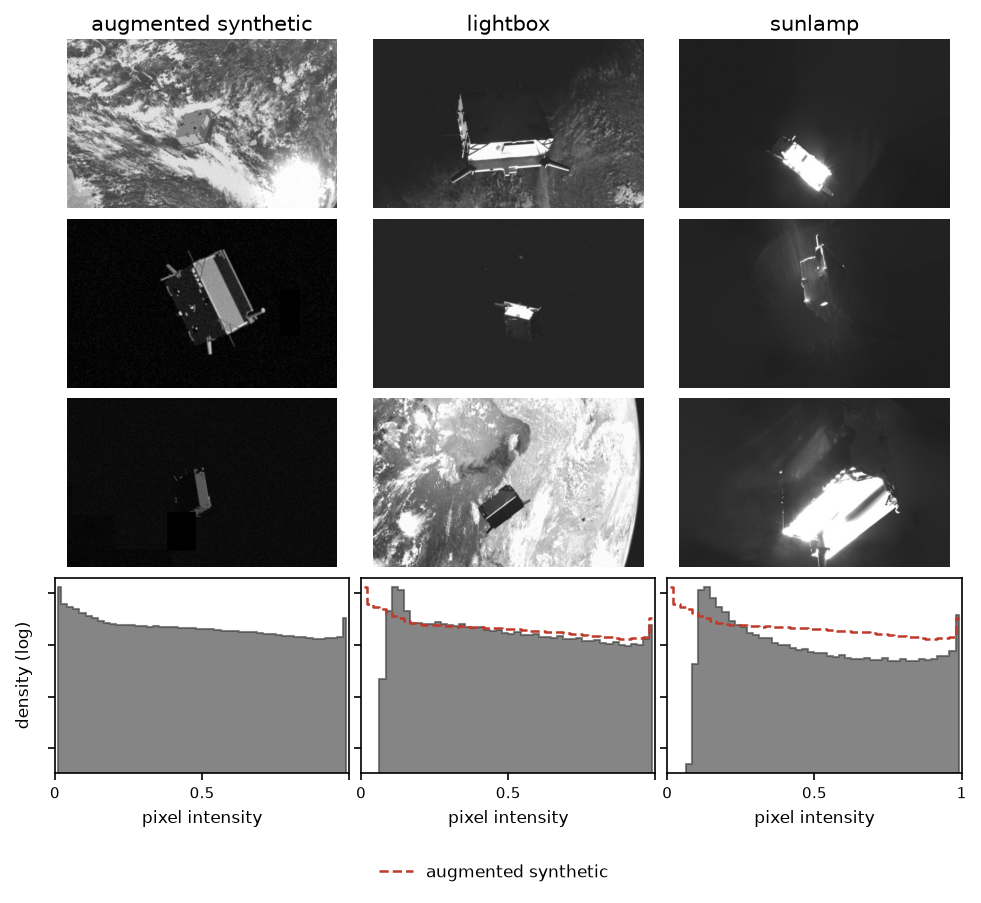
\includegraphics[width=\linewidth]{figures/crops_triptych_poolall.png}
  \end{minipage}\hfill
  \begin{minipage}[c]{0.49\linewidth}
    \caption{What the augmentation actually models. Columns: augmented synthetic training
  samples, and real test samples from each domain. Below each is the pixel-intensity
  density (log counts), pooled over every image in that split. The augmented density is
  overlaid on both real columns (dashed): far from both, and closer to lightbox---total
  variation $0.63$ against $0.80$. Gradient statistics give the same ordering
  (App.~\ref{app:revision}).}
    \label{fig:crops}
  \end{minipage}
\end{figure}

\emph{Mechanism.} The stack models \emph{diffuse} illumination variation: jitter and a
soft clamped blob simulate gentle, spatially smooth lighting change, which is what
lightbox is. Sunlamp is not: a collimated beam produces highlights off metallic and
foil surfaces, cast shadows, and \emph{clipped} regions. Photometric jitter only
brightens smoothly: the augmented images end up brighter overall than either real
domain, yet clip less often than sunlamp (2.0\% of pixels against 2.8\%). We expected
blur, noise and the glare blob to work against sunlamp's sharp, bright structure; the
ablation does not confirm this, and per-pixel gradients do not show sunlamp as sharper,
since most of its frame is dark (edge density 2.0\%, against 6.6\% for lightbox and
10.7\% for the augmented stack). Gradients do show direction: un-augmented synthetic
images are closer to lightbox than to sunlamp (gradient total variation 0.07 against
0.26), and the stack, mostly through blur and noise, pushes them away from both (0.29
and 0.51). Finally, layer 4's BatchNorm statistics track the augmented synthetic distribution, which
fits neither real domain well and lightbox less badly (Fig.~\ref{fig:crops}).
Augmentation pushed training toward the domain it was already least wrong about. Domain
randomization~\citep{tobin2017domainrand} helps where it brackets the target domain; ours
brackets neither, and misses sunlamp by more.

\subsection{The model does not know it is failing}
\label{sec:conformal}

Does the estimator's uncertainty survive the shift? We calibrate split conformal
regions~\citep{vovk2005algorithmic,lei2018distribution,angelopoulos2023gentle} per arm on
1{,}000 fresh synthetic images, used neither for training nor for checkpoint selection.
The score is Euclidean metres for translation (a keep-out sphere) and geodesic angle for
rotation (a cone), with the finite-sample-corrected quantile. At nominal 90\%, in-domain test coverage is close to nominal for every
arm and metric (87.7--91.4\%); its Clopper--Pearson~\citep{clopper1934use} intervals
include 90\% in every case but one, the frozen no-augmentation arm's translation
(87.7\%, 85.5--89.7\%), which is slightly anti-conservative. On the real domains it collapses. For the seeded no-augmentation
arms, rotation coverage is 9--13\% on sunlamp and 21--27\% on lightbox (translation
14--18\% / 33--35\%); App.~\ref{app:conformal} gives every arm, domain and seed, with
Clopper--Pearson intervals and inflation factors. Restoring 90\% rotation coverage on
sunlamp would mean inflating these arms' attitude cone ${\sim}5$--$6\times$, from ${\sim}0.5$ to
${\sim}2.8$\,rad---a cone holding roughly 78\% of all
orientations.\footnote{The fraction of $SO(3)$ lying within geodesic angle
$\alpha$ of a fixed rotation is $F(\alpha) = (\alpha - \sin\alpha)/\pi$; so
$F(2.79) \approx 0.78$, and $F(2.30)$ to $F(2.42)$ span $0.49$ to $0.56$.}
Coverage mirrors the directional finding of
Sec.~\ref{sec:directional}, where augmentation increases lightbox rotation coverage to
33--38\% but sunlamp only to 13--15\%. The frozen arms fail the opposite
way: their 90\% attitude cone already spans 2.30--2.42\,rad---49--56\% of
\emph{all possible orientations}---valid in-domain, but operationally meaningless.
A navigation filter fed these poses in deployment would receive wrong inputs that look
exactly as confident as correct ones (Fig.~\ref{fig:reliability}).
Test-time adaptation does not rescue this: re-estimating layer 4's BatchNorm statistics
on unlabelled real images (AdaBN~\citep{li2018adabn}; App.~\ref{app:revision}) lowers
rotation error on every layer-4 checkpoint (on average by 0.09\,rad on lightbox, 0.16
on sunlamp), yet rotation coverage reaches only 24--40\% and 11--20\%.

\begin{figure}[t]
  \centering
  \begin{minipage}[c]{0.37\linewidth}
    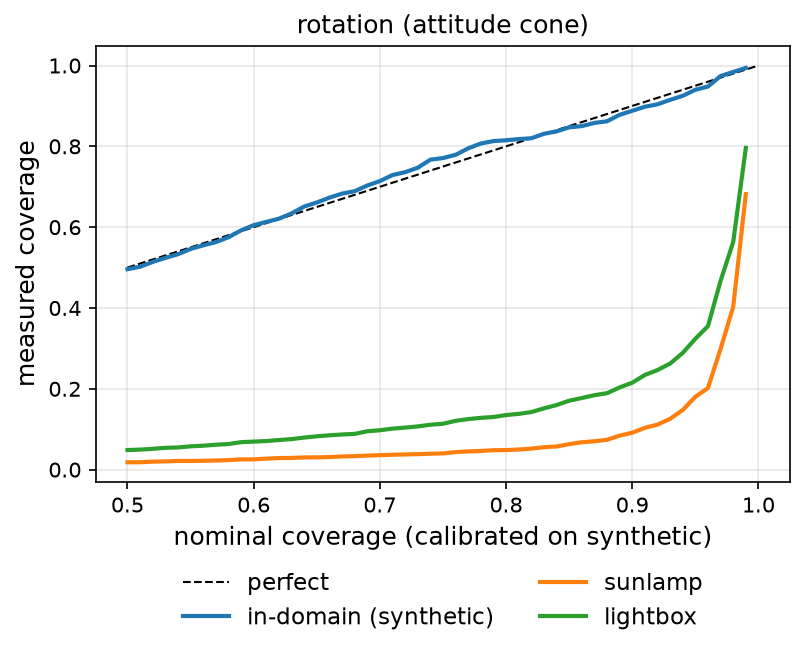
\includegraphics[width=\linewidth]{figures/reliability_unfrozen_no_aug_seed42_rotation.png}
  \end{minipage}\hfill
  \begin{minipage}[c]{0.59\linewidth}
    \caption{Conformal reliability of the attitude cone, layer 4
  no-augmentation arm (seed 42). In-domain coverage tracks the diagonal; both
  real domains collapse far below it. The guarantee is intact---exchangeability
  is what broke.}
    \label{fig:reliability}
  \end{minipage}
  % NOTE: seed-naming title already cropped out of the PNG.
\end{figure}

\section{Discussion and limitations}
\label{sec:discussion}

\paragraph{Ratios flatter weak models.} A degradation ratio divides by in-domain error:
on sunlamp even the skill-free constant pose (App.~\ref{app:constant}) scores only
$7.3\times$ our synthetic $S$, so our modest ratio does not mean a small gap. Nor do the
2019 results separate method classes: PnP entries in the top ten degraded
$4.8$--$40\times$, the others $2.7$--$24\times$~\citep{kisantal2020speed}. SPNv2~\citep{park2024spnv2}, the reference sim-to-real
method on SPEED+, closes far more of the gap with multi-task representations and heavy
style augmentation; we characterise how gains transfer under a simple estimator rather
than compete with it.

\paragraph{Limitations.} The frozen un-augmented arm was trained end to end on one seed,
the ablation arms and two frozen augmented seeds on different hardware from the
published ones, and sunlamp is the smaller
test set (2{,}791 images): three seeds do not resolve sunlamp effects of 0.1\,rad. We
study one estimator on one benchmark, at $320{\times}512$; with real-domain errors near
1\,rad this is a diagnostic baseline, not a deployable navigator. Our directionality
claim is about the match between an augmentation and the shift it faces, not about
photometric augmentation in general, and our image statistics pool whole frames, which
dark background dominates; object-masked statistics would test the mechanism more
directly. Our conformal coverage is also marginal rather than conditional: fixed
metre-radius spheres under-cover distant targets even in-domain, and range-normalising
overcorrects.

\paragraph{Future work.} The mechanism suggests its own tests: augmentation modelling
sunlamp's actual structure (specular highlights, hard shadows, saturation clipping), full
fine-tuning, and weighted conformal prediction~\citep{tibshirani2019covariate}, which
needs density ratios between domains that barely overlap---exactly what sim-to-real lacks.

For fields that must rely on synthetic data, ask of a robustness intervention not
``how much does it help?'' but ``which way does it push the training distribution?'';
and validate uncertainty under the shift, or a wrong pose arrives wrapped in a confident
interval.


\bibliographystyle{plainnat}
\bibliography{references}

% Reproducibility checklist. Sim2Science CFP: "placed after the references and before
% the appendix; it does not count toward the page limit. Missing or incomplete
% checklists may lead to desk rejection." Any appendix (S10) goes BELOW this input.
\newpage
\section*{NeurIPS Paper Checklist}




\begin{enumerate}

\item {\bf Claims}
    \item[] Question: Do the main claims made in the abstract and introduction accurately reflect the paper's contributions and scope?
    \item[] Answer: \answerYes{}
    \item[] Justification: The abstract and Section~\ref{sec:intro} state three findings---asymmetric transfer of
    synthetic gains, directionality of photometric augmentation, and the collapse of
    conformally calibrated coverage on the real domains---and each is supported by the
    corresponding results subsection (Sections~\ref{sec:asymmetry}, \ref{sec:directional},
    \ref{sec:conformal}) and by Table~\ref{tab:results}. The scope is stated explicitly: a
    single direct-regression baseline on SPEED+, characterising transfer \emph{structure}
    rather than competing with state-of-the-art sim-to-real pipelines
    (Section~\ref{sec:discussion}).
    \item[] Guidelines:
    \begin{itemize}
        \item The answer \answerNA{} means that the abstract and introduction do not include the claims made in the paper.
        \item The abstract and/or introduction should clearly state the claims made, including the contributions made in the paper and important assumptions and limitations. A \answerNo{} or \answerNA{} answer to this question will not be perceived well by the reviewers. 
        \item The claims made should match theoretical and experimental results, and reflect how much the results can be expected to generalize to other settings. 
        \item It is fine to include aspirational goals as motivation as long as it is clear that these goals are not attained by the paper. 
    \end{itemize}

\item {\bf Limitations}
    \item[] Question: Does the paper discuss the limitations of the work performed by the authors?
    \item[] Answer: \answerYes{}
    \item[] Justification: Section~\ref{sec:discussion} contains a dedicated ``Limitations'' paragraph: the
    frozen un-augmented arm was trained end to end on one seed (its seed spread comes from head-only
    retrains), and the ablation arms and two frozen augmented seeds ran on different hardware; sunlamp is the smaller test
    set (2{,}791 images) and therefore noisier; the study covers one estimator on one
    benchmark at reduced resolution; the directionality claim is scoped to one augmentation stack against
    one shift, not to photometric augmentation in general; the image statistics pool whole
    frames, which dark background dominates; and
    the conformal coverage reported is marginal rather than conditional. The same section also
    states that the modest relative degradation is a property of the direct-regression method
    class and is \emph{not} evidence of a small sim-to-real gap.
    \item[] Guidelines:
    \begin{itemize}
        \item The answer \answerNA{} means that the paper has no limitation while the answer \answerNo{} means that the paper has limitations, but those are not discussed in the paper. 
        \item The authors are encouraged to create a separate ``Limitations'' section in their paper.
        \item The paper should point out any strong assumptions and how robust the results are to violations of these assumptions (e.g., independence assumptions, noiseless settings, model well-specification, asymptotic approximations only holding locally). The authors should reflect on how these assumptions might be violated in practice and what the implications would be.
        \item The authors should reflect on the scope of the claims made, e.g., if the approach was only tested on a few datasets or with a few runs. In general, empirical results often depend on implicit assumptions, which should be articulated.
        \item The authors should reflect on the factors that influence the performance of the approach. For example, a facial recognition algorithm may perform poorly when image resolution is low or images are taken in low lighting. Or a speech-to-text system might not be used reliably to provide closed captions for online lectures because it fails to handle technical jargon.
        \item The authors should discuss the computational efficiency of the proposed algorithms and how they scale with dataset size.
        \item If applicable, the authors should discuss possible limitations of their approach to address problems of privacy and fairness.
        \item While the authors might fear that complete honesty about limitations might be used by reviewers as grounds for rejection, a worse outcome might be that reviewers discover limitations that aren't acknowledged in the paper. The authors should use their best judgment and recognize that individual actions in favor of transparency play an important role in developing norms that preserve the integrity of the community. Reviewers will be specifically instructed to not penalize honesty concerning limitations.
    \end{itemize}

\item {\bf Theory assumptions and proofs}
    \item[] Question: For each theoretical result, does the paper provide the full set of assumptions and a complete (and correct) proof?
    \item[] Answer: \answerNA{}
    \item[] Justification: The paper contains no theorems or new theoretical results. It uses two
    closed-form expressions, both standard: the mean geodesic angle under the Haar measure
    on $SO(3)$ ($\pi/2 + \nicefrac{2}{\pi}$, Section~\ref{sec:setup}) and the volume
    fraction $F(\alpha) = (\alpha - \sin\alpha)/\pi$ (Section~\ref{sec:conformal}). The
    density they follow from is stated inline.
    \item[] Guidelines:
    \begin{itemize}
        \item The answer \answerNA{} means that the paper does not include theoretical results. 
        \item All the theorems, formulas, and proofs in the paper should be numbered and cross-referenced.
        \item All assumptions should be clearly stated or referenced in the statement of any theorems.
        \item The proofs can either appear in the main paper or the supplemental material, but if they appear in the supplemental material, the authors are encouraged to provide a short proof sketch to provide intuition. 
        \item Inversely, any informal proof provided in the core of the paper should be complemented by formal proofs provided in appendix or supplemental material.
        \item Theorems and Lemmas that the proof relies upon should be properly referenced. 
    \end{itemize}

    \item {\bf Experimental result reproducibility}
    \item[] Question: Does the paper fully disclose all the information needed to reproduce the main experimental results of the paper to the extent that it affects the main claims and/or conclusions of the paper (regardless of whether the code and data are provided or not)?
    \item[] Answer: \answerYes{}
    \item[] Justification: Section~\ref{sec:setup} discloses the data splits: 28{,}000 synthetic training
    and 2{,}000 synthetic validation images, plus the full lightbox and sunlamp sets
    (6{,}740 and 2{,}791 images) used only as test sets. It also gives the preprocessing
    ($320{\times}512$ grayscale), the architecture and head, the loss including $\lambda$ and
    the quaternion canonicalisation, the optimiser and every training hyperparameter, the
    checkpoint-selection rule, the seeds, the full augmentation ranges and probabilities, and
    the metric definitions. Section~\ref{sec:conformal} specifies the conformal protocol:
    split conformal at nominal 90\%, calibrated per arm on 1{,}000 fresh synthetic images
    never used for training or checkpoint selection, with a finite-sample-corrected quantile
    and the score function used for each of translation and rotation.
    \item[] Guidelines:
    \begin{itemize}
        \item The answer \answerNA{} means that the paper does not include experiments.
        \item If the paper includes experiments, a \answerNo{} answer to this question will not be perceived well by the reviewers: Making the paper reproducible is important, regardless of whether the code and data are provided or not.
        \item If the contribution is a dataset and\slash or model, the authors should describe the steps taken to make their results reproducible or verifiable. 
        \item Depending on the contribution, reproducibility can be accomplished in various ways. For example, if the contribution is a novel architecture, describing the architecture fully might suffice, or if the contribution is a specific model and empirical evaluation, it may be necessary to either make it possible for others to replicate the model with the same dataset, or provide access to the model. In general. releasing code and data is often one good way to accomplish this, but reproducibility can also be provided via detailed instructions for how to replicate the results, access to a hosted model (e.g., in the case of a large language model), releasing of a model checkpoint, or other means that are appropriate to the research performed.
        \item While NeurIPS does not require releasing code, the conference does require all submissions to provide some reasonable avenue for reproducibility, which may depend on the nature of the contribution. For example
        \begin{enumerate}
            \item If the contribution is primarily a new algorithm, the paper should make it clear how to reproduce that algorithm.
            \item If the contribution is primarily a new model architecture, the paper should describe the architecture clearly and fully.
            \item If the contribution is a new model (e.g., a large language model), then there should either be a way to access this model for reproducing the results or a way to reproduce the model (e.g., with an open-source dataset or instructions for how to construct the dataset).
            \item We recognize that reproducibility may be tricky in some cases, in which case authors are welcome to describe the particular way they provide for reproducibility. In the case of closed-source models, it may be that access to the model is limited in some way (e.g., to registered users), but it should be possible for other researchers to have some path to reproducing or verifying the results.
        \end{enumerate}
    \end{itemize}


\item {\bf Open access to data and code}
    \item[] Question: Does the paper provide open access to the data and code, with sufficient instructions to faithfully reproduce the main experimental results, as described in supplemental material?
    \item[] Answer: \answerYes{}
    \item[] Justification: SPEED+~\citep{park2022speedplus} is a public benchmark obtained from its official host.
    The code, configuration, per-seed results, and conformal analysis behind every number
    reported here are in the public repository linked in the ``Code and data''
    paragraph of Section~\ref{sec:setup}.
    \item[] Guidelines:
    \begin{itemize}
        \item The answer \answerNA{} means that paper does not include experiments requiring code.
        \item Please see the NeurIPS code and data submission guidelines (\url{https://neurips.cc/public/guides/CodeSubmissionPolicy}) for more details.
        \item While we encourage the release of code and data, we understand that this might not be possible, so \answerNo{} is an acceptable answer. Papers cannot be rejected simply for not including code, unless this is central to the contribution (e.g., for a new open-source benchmark).
        \item The instructions should contain the exact command and environment needed to run to reproduce the results. See the NeurIPS code and data submission guidelines (\url{https://neurips.cc/public/guides/CodeSubmissionPolicy}) for more details.
        \item The authors should provide instructions on data access and preparation, including how to access the raw data, preprocessed data, intermediate data, and generated data, etc.
        \item The authors should provide scripts to reproduce all experimental results for the new proposed method and baselines. If only a subset of experiments are reproducible, they should state which ones are omitted from the script and why.
        \item At submission time, to preserve anonymity, the authors should release anonymized versions (if applicable).
        \item Providing as much information as possible in supplemental material (appended to the paper) is recommended, but including URLs to data and code is permitted.
    \end{itemize}


\item {\bf Experimental setting/details}
    \item[] Question: Does the paper specify all the training and test details (e.g., data splits, hyperparameters, how they were chosen, type of optimizer) necessary to understand the results?
    \item[] Answer: \answerYes{}
    \item[] Justification: Section~\ref{sec:setup} specifies the splits, the optimiser (Adam), learning rate
    ($10^{-3}$), batch size (16), 20 epochs with checkpoints on even epochs, $\lambda{=}1$,
    per-component z-scoring of translation targets, and the seeds $\{42,43,44\}$. Model
    selection is by best \emph{synthetic} validation rotation error, applied uniformly across
    all arms. Hyperparameters were not tuned per arm: the configuration is held fixed across
    the whole $2{\times}2$ design, so the comparison is like-for-like. No real image
    influenced training, tuning, or model selection.
    \item[] Guidelines:
    \begin{itemize}
        \item The answer \answerNA{} means that the paper does not include experiments.
        \item The experimental setting should be presented in the core of the paper to a level of detail that is necessary to appreciate the results and make sense of them.
        \item The full details can be provided either with the code, in appendix, or as supplemental material.
    \end{itemize}

\item {\bf Experiment statistical significance}
    \item[] Question: Does the paper report error bars suitably and correctly defined or other appropriate information about the statistical significance of the experiments?
    \item[] Answer: \answerYes{}
    \item[] Justification: Three of the four arms are run on three seeds and reported as mean $\pm$ one standard
    deviation in Table~\ref{tab:results}, with all 30 per-seed values
    in App.~\ref{app:perseed}. Because seeds are paired across arms,
    Section~\ref{sec:directional} reads seed-paired differences rather than comparing spreads,
    and states the sign of every paired difference. Conformal coverage is reported with
    Clopper--Pearson binomial confidence intervals~\citep{clopper1934use}. The frozen un-augmented arm was
    trained end to end on one seed, marked $\dagger$ in Table~\ref{tab:results}; three-seed
    head-only retrains give its spread (App.~\ref{app:revision}), and the ablation arms are
    read as seed-paired differences against a same-hardware control.
    The variability captured is over the random seed (head initialisation, data ordering, and
    augmentation sampling).
    \item[] Guidelines:
    \begin{itemize}
        \item The answer \answerNA{} means that the paper does not include experiments.
        \item The authors should answer \answerYes{} if the results are accompanied by error bars, confidence intervals, or statistical significance tests, at least for the experiments that support the main claims of the paper.
        \item The factors of variability that the error bars are capturing should be clearly stated (for example, train/test split, initialization, random drawing of some parameter, or overall run with given experimental conditions).
        \item The method for calculating the error bars should be explained (closed form formula, call to a library function, bootstrap, etc.)
        \item The assumptions made should be given (e.g., Normally distributed errors).
        \item It should be clear whether the error bar is the standard deviation or the standard error of the mean.
        \item It is OK to report 1-sigma error bars, but one should state it. The authors should preferably report a 2-sigma error bar than state that they have a 96\% CI, if the hypothesis of Normality of errors is not verified.
        \item For asymmetric distributions, the authors should be careful not to show in tables or figures symmetric error bars that would yield results that are out of range (e.g., negative error rates).
        \item If error bars are reported in tables or plots, the authors should explain in the text how they were calculated and reference the corresponding figures or tables in the text.
    \end{itemize}

\item {\bf Experiments compute resources}
    \item[] Question: For each experiment, does the paper provide sufficient information on the computer resources (type of compute workers, memory, time of execution) needed to reproduce the experiments?
    \item[] Answer: \answerYes{}
    \item[] Justification: All training was done on a single cloud-hosted consumer-class GPU (Google Colab), which is
    why images are downscaled to $320{\times}512$ grayscale (Section~\ref{sec:setup}). A
    20-epoch run takes 320--355\,s per epoch without augmentation and 780--795\,s per
    epoch with it, i.e.\ about 1.8--2.0\,h and 4.3--4.4\,h per run: the augmentation
    pipeline dominates, and frozen and unfrozen arms differ by under 10\%. The eight
    Colab training runs behind Table~\ref{tab:results} (four augmented, four not) total
    roughly 25 GPU-hours. Evaluation
    and conformal calibration are inference-only and take a few minutes per checkpoint.
    The revision experiments (App.~\ref{app:revision}) ran on an Apple M5 laptop GPU:
    each of the seven layer-4 runs took about 3.7\,h (about 26\,h in total), the two
    frozen augmented runs in Table~\ref{tab:results} about 3.2\,h each, the
    cached-feature heads a few minutes each on CPU, and AdaBN and the image statistics
    under an hour together.
    \item[] Guidelines:
    \begin{itemize}
        \item The answer \answerNA{} means that the paper does not include experiments.
        \item The paper should indicate the type of compute workers CPU or GPU, internal cluster, or cloud provider, including relevant memory and storage.
        \item The paper should provide the amount of compute required for each of the individual experimental runs as well as estimate the total compute. 
        \item The paper should disclose whether the full research project required more compute than the experiments reported in the paper (e.g., preliminary or failed experiments that didn't make it into the paper). 
    \end{itemize}
    
\item {\bf Code of ethics}
    \item[] Question: Does the research conducted in the paper conform, in every respect, with the NeurIPS Code of Ethics \url{https://neurips.cc/public/EthicsGuidelines}?
    \item[] Answer: \answerYes{}
    \item[] Justification: The research uses a public benchmark of a spacecraft mockup. It involves no human
    subjects, no personal or personally identifiable data, and no scraped or crowdsourced
    content. The assets used are credited and used under their terms.
    \item[] Guidelines:
    \begin{itemize}
        \item The answer \answerNA{} means that the authors have not reviewed the NeurIPS Code of Ethics.
        \item If the authors answer \answerNo, they should explain the special circumstances that require a deviation from the Code of Ethics.
        \item The authors should make sure to preserve anonymity (e.g., if there is a special consideration due to laws or regulations in their jurisdiction).
    \end{itemize}


\item {\bf Broader impacts}
    \item[] Question: Does the paper discuss both potential positive societal impacts and negative societal impacts of the work performed?
    \item[] Answer: \answerYes{}
    \item[] Justification: The positive motivation---vision-based navigation for on-orbit servicing, inspection, and
    debris removal---is stated in Section~\ref{sec:intro}. The negative-impact side is the
    paper's third finding and is stated operationally in Sections~\ref{sec:conformal}
    and~\ref{sec:discussion}: a pose estimator whose uncertainty was calibrated on the
    simulator emits wrong poses carrying the confidence of correct ones, so a downstream
    navigation filter is silently misled. Naming that failure mode is the paper's main safety
    contribution. No new capability with dual-use potential is released.
    \item[] Guidelines:
    \begin{itemize}
        \item The answer \answerNA{} means that there is no societal impact of the work performed.
        \item If the authors answer \answerNA{} or \answerNo, they should explain why their work has no societal impact or why the paper does not address societal impact.
        \item Examples of negative societal impacts include potential malicious or unintended uses (e.g., disinformation, generating fake profiles, surveillance), fairness considerations (e.g., deployment of technologies that could make decisions that unfairly impact specific groups), privacy considerations, and security considerations.
        \item The conference expects that many papers will be foundational research and not tied to particular applications, let alone deployments. However, if there is a direct path to any negative applications, the authors should point it out. For example, it is legitimate to point out that an improvement in the quality of generative models could be used to generate Deepfakes for disinformation. On the other hand, it is not needed to point out that a generic algorithm for optimizing neural networks could enable people to train models that generate Deepfakes faster.
        \item The authors should consider possible harms that could arise when the technology is being used as intended and functioning correctly, harms that could arise when the technology is being used as intended but gives incorrect results, and harms following from (intentional or unintentional) misuse of the technology.
        \item If there are negative societal impacts, the authors could also discuss possible mitigation strategies (e.g., gated release of models, providing defenses in addition to attacks, mechanisms for monitoring misuse, mechanisms to monitor how a system learns from feedback over time, improving the efficiency and accessibility of ML).
    \end{itemize}
    
\item {\bf Safeguards}
    \item[] Question: Does the paper describe safeguards that have been put in place for responsible release of data or models that have a high risk for misuse (e.g., pre-trained language models, image generators, or scraped datasets)?
    \item[] Answer: \answerNA{}
    \item[] Justification: No data or models with a high risk of misuse are released. The released artefact is a
    small pose-regression baseline on a public benchmark, deliberately below the state of the
    art, together with the analysis code that reproduces the reported numbers.
    \item[] Guidelines:
    \begin{itemize}
        \item The answer \answerNA{} means that the paper poses no such risks.
        \item Released models that have a high risk for misuse or dual-use should be released with necessary safeguards to allow for controlled use of the model, for example by requiring that users adhere to usage guidelines or restrictions to access the model or implementing safety filters. 
        \item Datasets that have been scraped from the Internet could pose safety risks. The authors should describe how they avoided releasing unsafe images.
        \item We recognize that providing effective safeguards is challenging, and many papers do not require this, but we encourage authors to take this into account and make a best faith effort.
    \end{itemize}

\item {\bf Licenses for existing assets}
    \item[] Question: Are the creators or original owners of assets (e.g., code, data, models), used in the paper, properly credited and are the license and terms of use explicitly mentioned and properly respected?
    \item[] Answer: \answerYes{}
    \item[] Justification: SPEED+ is cited to its dataset paper and challenge
    report~\citep{park2022speedplus,kisantal2020speed} and was obtained from its official
    Zenodo record, which distributes it under the Creative Commons Attribution 4.0
    International (CC BY 4.0) licence; it is used under those terms and is not
    redistributed here. The backbone is the torchvision ResNet-50~\citep{he2016resnet}
    (code under BSD-3-Clause; the pretrained weights under torchvision's terms)
    pretrained on ImageNet~\citep{deng2009imagenet}, both
    cited. Methodological antecedents for direct pose regression and split conformal
    prediction are cited in Sections~\ref{sec:setup} and~\ref{sec:conformal}.
    \item[] Guidelines:
    \begin{itemize}
        \item The answer \answerNA{} means that the paper does not use existing assets.
        \item The authors should cite the original paper that produced the code package or dataset.
        \item The authors should state which version of the asset is used and, if possible, include a URL.
        \item The name of the license (e.g., CC-BY 4.0) should be included for each asset.
        \item For scraped data from a particular source (e.g., website), the copyright and terms of service of that source should be provided.
        \item If assets are released, the license, copyright information, and terms of use in the package should be provided. For popular datasets, \url{paperswithcode.com/datasets} has curated licenses for some datasets. Their licensing guide can help determine the license of a dataset.
        \item For existing datasets that are re-packaged, both the original license and the license of the derived asset (if it has changed) should be provided.
        \item If this information is not available online, the authors are encouraged to reach out to the asset's creators.
    \end{itemize}

\item {\bf New assets}
    \item[] Question: Are new assets introduced in the paper well documented and is the documentation provided alongside the assets?
    \item[] Answer: \answerNA{}
    \item[] Justification: The paper introduces no new dataset, benchmark, or pretrained model. The accompanying
    code is a public repository of the experiment and analysis code that reproduces the
    reported numbers, documented by a README; it is a reproduction artefact rather than a new
    released asset.
    \item[] Guidelines:
    \begin{itemize}
        \item The answer \answerNA{} means that the paper does not release new assets.
        \item Researchers should communicate the details of the dataset\slash code\slash model as part of their submissions via structured templates. This includes details about training, license, limitations, etc. 
        \item The paper should discuss whether and how consent was obtained from people whose asset is used.
        \item At submission time, remember to anonymize your assets (if applicable). You can either create an anonymized URL or include an anonymized zip file.
    \end{itemize}

\item {\bf Crowdsourcing and research with human subjects}
    \item[] Question: For crowdsourcing experiments and research with human subjects, does the paper include the full text of instructions given to participants and screenshots, if applicable, as well as details about compensation (if any)? 
    \item[] Answer: \answerNA{}
    \item[] Justification: The paper involves no crowdsourcing and no research with human subjects.
    \item[] Guidelines:
    \begin{itemize}
        \item The answer \answerNA{} means that the paper does not involve crowdsourcing nor research with human subjects.
        \item Including this information in the supplemental material is fine, but if the main contribution of the paper involves human subjects, then as much detail as possible should be included in the main paper. 
        \item According to the NeurIPS Code of Ethics, workers involved in data collection, curation, or other labor should be paid at least the minimum wage in the country of the data collector. 
    \end{itemize}

\item {\bf Institutional review board (IRB) approvals or equivalent for research with human subjects}
    \item[] Question: Does the paper describe potential risks incurred by study participants, whether such risks were disclosed to the subjects, and whether Institutional Review Board (IRB) approvals (or an equivalent approval/review based on the requirements of your country or institution) were obtained?
    \item[] Answer: \answerNA{}
    \item[] Justification: The paper involves no research with human subjects, so no IRB or equivalent review was
    required.
    \item[] Guidelines:
    \begin{itemize}
        \item The answer \answerNA{} means that the paper does not involve crowdsourcing nor research with human subjects.
        \item Depending on the country in which research is conducted, IRB approval (or equivalent) may be required for any human subjects research. If you obtained IRB approval, you should clearly state this in the paper. 
        \item We recognize that the procedures for this may vary significantly between institutions and locations, and we expect authors to adhere to the NeurIPS Code of Ethics and the guidelines for their institution. 
        \item For initial submissions, do not include any information that would break anonymity (if applicable), such as the institution conducting the review.
    \end{itemize}

\item {\bf Declaration of LLM usage}
    \item[] Question: Does the paper describe the usage of LLMs if it is an important, original, or non-standard component of the core methods in this research? Note that if the LLM is used only for writing, editing, or formatting purposes and does \emph{not} impact the core methodology, scientific rigor, or originality of the research, declaration is not required.
    %this research? 
    \item[] Answer: \answerNA{}
    \item[] Justification: No large language model is a component of the method: the estimator is a ResNet-50 with a
    small regression head. LLM assistance was limited to writing and editing, which, per the
    question above and the NeurIPS policy on LLM use, does not require declaration.
    \item[] Guidelines:
    \begin{itemize}
        \item The answer \answerNA{} means that the core method development in this research does not involve LLMs as any important, original, or non-standard components.
        \item Please refer to our LLM policy in the NeurIPS handbook for what should or should not be described.
    \end{itemize}

\end{enumerate}

% ---- Appendix: after the checklist, per the Sim2Science CFP ----
\newpage
% =========================================================================
% Appendix. Sits after the reproducibility checklist, per the Sim2Science CFP.
% GENERATED by make_appendix.py from project_context/results_table.md.
% Edit the generator, not this file.
% =========================================================================
\appendix

\section{Per-seed results}
\label{app:perseed}

Table~\ref{tab:perseed} lists every run behind Table~\ref{tab:results}: all 30
arm\,$\times$\,seed\,$\times$\,domain evaluations. The frozen un-augmented arm was run on
seed 42 only, the other arms on seeds 42, 43 and 44; frozen augmented seeds 43 and 44
were trained on an Apple M5 (App.~\ref{app:revision}). Each run keeps the checkpoint with the best
\emph{synthetic} validation rotation error, chosen without reference to either real
domain.

\begin{table}[ht]
  \caption{Per-seed results. $\Etrans$ is range-normalised; $\Erot$ is geodesic
  rotation error in radians (chance level 2.207).}
  \label{tab:perseed}
  \centering
  \small
  \begin{tabular}{ll c l cc}
    \toprule
    Backbone & Aug. & Seed & Domain & $\Etrans$ & $\Erot$ \\
    \midrule
    frozen & -- & 42 & synthetic (val) & 0.066 & 1.053 \\
    frozen & -- & 42 & sunlamp & 0.253 & 2.048 \\
    frozen & -- & 42 & lightbox & 0.151 & 1.752 \\
    \midrule
    frozen & \checkmark & 42 & synthetic (val) & 0.071 & 1.180 \\
    frozen & \checkmark & 42 & sunlamp & 0.306 & 1.864 \\
    frozen & \checkmark & 42 & lightbox & 0.118 & 1.718 \\
    frozen & \checkmark & 43 & synthetic (val) & 0.073 & 1.205 \\
    frozen & \checkmark & 43 & sunlamp & 0.328 & 1.883 \\
    frozen & \checkmark & 43 & lightbox & 0.126 & 1.734 \\
    frozen & \checkmark & 44 & synthetic (val) & 0.074 & 1.169 \\
    frozen & \checkmark & 44 & sunlamp & 0.279 & 1.881 \\
    frozen & \checkmark & 44 & lightbox & 0.118 & 1.673 \\
    \midrule
    layer 4 & -- & 42 & synthetic (val) & 0.039 & 0.306 \\
    layer 4 & -- & 42 & sunlamp & 0.299 & 1.476 \\
    layer 4 & -- & 42 & lightbox & 0.200 & 1.169 \\
    layer 4 & -- & 43 & synthetic (val) & 0.035 & 0.326 \\
    layer 4 & -- & 43 & sunlamp & 0.352 & 1.619 \\
    layer 4 & -- & 43 & lightbox & 0.152 & 1.182 \\
    layer 4 & -- & 44 & synthetic (val) & 0.035 & 0.318 \\
    layer 4 & -- & 44 & sunlamp & 0.283 & 1.506 \\
    layer 4 & -- & 44 & lightbox & 0.154 & 1.147 \\
    \midrule
    layer 4 & \checkmark & 42 & synthetic (val) & 0.041 & 0.352 \\
    layer 4 & \checkmark & 42 & sunlamp & 0.405 & 1.592 \\
    layer 4 & \checkmark & 42 & lightbox & 0.152 & 0.986 \\
    layer 4 & \checkmark & 43 & synthetic (val) & 0.044 & 0.302 \\
    layer 4 & \checkmark & 43 & sunlamp & 0.399 & 1.354 \\
    layer 4 & \checkmark & 43 & lightbox & 0.165 & 0.997 \\
    layer 4 & \checkmark & 44 & synthetic (val) & 0.042 & 0.311 \\
    layer 4 & \checkmark & 44 & sunlamp & 0.261 & 1.459 \\
    layer 4 & \checkmark & 44 & lightbox & 0.132 & 0.977 \\
    \bottomrule
  \end{tabular}
\end{table}

\section{Conformal coverage, all arms and domains}
\label{app:conformal}

Split-conformal regions are calibrated per arm on 1{,}000 held-out synthetic images
used neither for training nor for checkpoint selection, at nominal 90\% coverage with
the finite-sample-corrected quantile. Coverage carries Clopper--Pearson 95\%
intervals~\citep{clopper1934use}. $\hat{q}$ is the calibrated region size: a keep-out
sphere radius for translation, a cone half-angle for rotation. \emph{Inflation} is the
factor by which $\hat{q}$ would have to grow to restore 90\% coverage on that domain, so
it measures directly how far the calibration is wrong. It sits near $1$ in-domain and
reaches $1.2$--$13\times$ on the real domains, worst on the sharper unfrozen arms. A low
factor on the frozen arms is not good news: their cones are already wide enough in-domain
to be uninformative. The ``synthetic (selection split)'' rows are the 2{,}000-image validation split used
for checkpoint selection, kept as a second, not fully independent, in-domain control.

Table~\ref{tab:conformal-abs} uses absolute scores: Euclidean metres for translation,
geodesic radians for rotation. Table~\ref{tab:conformal-rel} repeats the translation
analysis under the range-normalised score reported in the body. The two disagree on
in-domain conditional behaviour---fixed metre spheres under-cover distant targets,
range-normalising overcorrects at short range---but the collapse on the real domains
is the same either way.

\begin{table}[ht]
  \caption{Conformal coverage at nominal 90\%, absolute scores. Coverage in \% with
  Clopper--Pearson 95\% intervals; $\hat{q}_T$ in metres, $\hat{q}_R$ in radians.}
  \label{tab:conformal-abs}
  \centering
  \scriptsize
  \setlength{\tabcolsep}{3pt}
  \begin{tabular}{ll c l ccc ccc}
    \toprule
    & & & & \multicolumn{3}{c}{Translation (sphere)} & \multicolumn{3}{c}{Rotation (cone)} \\
    \cmidrule(lr){5-7} \cmidrule(lr){8-10}
    Backbone & Aug. & Seed & Domain & Cov. & $\hat{q}_T$ & Infl. & Cov. & $\hat{q}_R$ & Infl. \\
    \midrule
    frozen & -- & 42 & synthetic (val) & 87.7 (85.5--89.7) & 0.712 & 1.11 & 90.0 (88.0--91.8) & 2.299 & 1.01 \\
    frozen & -- & 42 & sunlamp & 29.2 (27.5--30.9) & 0.712 & 4.76 & 58.2 (56.3--60.0) & 2.299 & 1.28 \\
    frozen & -- & 42 & lightbox & 52.1 (50.9--53.3) & 0.712 & 2.48 & 71.0 (69.9--72.1) & 2.299 & 1.24 \\
    frozen & -- & 42 & synthetic (selection split) & 88.0 (86.5--89.4) & 0.712 & 1.08 & 90.5 (89.1--91.7) & 2.299 & 0.99 \\
    \midrule
    frozen & \checkmark & 42 & synthetic (val) & 89.3 (87.2--91.1) & 0.793 & 1.01 & 88.7 (86.6--90.6) & 2.403 & 1.02 \\
    frozen & \checkmark & 42 & sunlamp & 26.3 (24.6--27.9) & 0.793 & 5.36 & 71.0 (69.3--72.7) & 2.403 & 1.20 \\
    frozen & \checkmark & 42 & lightbox & 68.3 (67.2--69.4) & 0.793 & 1.84 & 75.1 (74.1--76.2) & 2.403 & 1.19 \\
    frozen & \checkmark & 42 & synthetic (selection split) & 89.9 (88.5--91.2) & 0.793 & 1.01 & 89.5 (88.0--90.8) & 2.403 & 1.02 \\
    frozen & \checkmark & 43 & synthetic (val) & 89.7 (87.6--91.5) & 0.828 & 1.01 & 90.9 (88.9--92.6) & 2.415 & 0.98 \\
    frozen & \checkmark & 43 & sunlamp & 23.4 (21.8--25.0) & 0.828 & 5.16 & 70.0 (68.3--71.7) & 2.415 & 1.20 \\
    frozen & \checkmark & 43 & lightbox & 66.9 (65.7--68.0) & 0.828 & 1.91 & 75.5 (74.4--76.5) & 2.415 & 1.18 \\
    frozen & \checkmark & 43 & synthetic (selection split) & 89.6 (88.2--91.0) & 0.828 & 1.01 & 88.9 (87.4--90.2) & 2.415 & 1.03 \\
    frozen & \checkmark & 44 & synthetic (val) & 89.8 (87.8--91.6) & 0.839 & 1.00 & 91.1 (89.2--92.8) & 2.372 & 0.97 \\
    frozen & \checkmark & 44 & sunlamp & 30.1 (28.4--31.9) & 0.839 & 4.69 & 69.8 (68.1--71.5) & 2.372 & 1.21 \\
    frozen & \checkmark & 44 & lightbox & 71.1 (70.0--72.2) & 0.839 & 1.72 & 76.3 (75.2--77.3) & 2.372 & 1.18 \\
    frozen & \checkmark & 44 & synthetic (selection split) & 89.8 (88.4--91.1) & 0.839 & 1.01 & 89.5 (88.1--90.8) & 2.372 & 1.01 \\
    \midrule
    layer 4 & -- & 42 & synthetic (val) & 89.3 (87.2--91.1) & 0.410 & 1.04 & 88.8 (86.7--90.7) & 0.460 & 1.06 \\
    layer 4 & -- & 42 & sunlamp & 18.2 (16.8--19.6) & 0.410 & 10.92 & 9.1 (8.1--10.3) & 0.460 & 6.07 \\
    layer 4 & -- & 42 & lightbox & 34.1 (32.9--35.2) & 0.410 & 7.92 & 21.5 (20.5--22.5) & 0.460 & 5.52 \\
    layer 4 & -- & 42 & synthetic (selection split) & 89.6 (88.2--90.9) & 0.410 & 1.01 & 87.2 (85.7--88.7) & 0.460 & 1.10 \\
    \midrule
    layer 4 & -- & 43 & synthetic (val) & 90.2 (88.2--92.0) & 0.378 & 0.99 & 89.1 (87.0--91.0) & 0.540 & 1.04 \\
    layer 4 & -- & 43 & sunlamp & 13.8 (12.6--15.2) & 0.378 & 13.42 & 9.0 (8.0--10.1) & 0.540 & 5.23 \\
    layer 4 & -- & 43 & lightbox & 35.4 (34.3--36.6) & 0.378 & 6.41 & 26.7 (25.6--27.7) & 0.540 & 4.76 \\
    layer 4 & -- & 43 & synthetic (selection split) & 89.2 (87.8--90.5) & 0.378 & 1.02 & 89.2 (87.8--90.5) & 0.540 & 1.05 \\
    \midrule
    layer 4 & -- & 44 & synthetic (val) & 89.9 (87.9--91.7) & 0.368 & 1.01 & 89.7 (87.6--91.5) & 0.526 & 1.02 \\
    layer 4 & -- & 44 & sunlamp & 18.0 (16.6--19.5) & 0.368 & 11.73 & 12.9 (11.7--14.2) & 0.526 & 5.30 \\
    layer 4 & -- & 44 & lightbox & 32.9 (31.8--34.1) & 0.368 & 6.52 & 26.5 (25.4--27.5) & 0.526 & 4.71 \\
    layer 4 & -- & 44 & synthetic (selection split) & 88.4 (87.0--89.8) & 0.368 & 1.05 & 90.5 (89.1--91.7) & 0.526 & 0.99 \\
    \midrule
    layer 4 & \checkmark & 42 & synthetic (val) & 89.8 (87.8--91.6) & 0.425 & 1.01 & 91.2 (89.3--92.9) & 0.576 & 0.97 \\
    layer 4 & \checkmark & 42 & sunlamp & 10.0 (8.9--11.2) & 0.425 & 12.79 & 12.6 (11.4--13.9) & 0.576 & 4.88 \\
    layer 4 & \checkmark & 42 & lightbox & 44.3 (43.1--45.5) & 0.425 & 6.45 & 37.2 (36.1--38.4) & 0.576 & 3.82 \\
    layer 4 & \checkmark & 42 & synthetic (selection split) & 89.8 (88.3--91.0) & 0.425 & 1.01 & 90.0 (88.7--91.3) & 0.576 & 1.00 \\
    \midrule
    layer 4 & \checkmark & 43 & synthetic (val) & 90.4 (88.4--92.2) & 0.494 & 0.98 & 91.1 (89.2--92.8) & 0.483 & 0.96 \\
    layer 4 & \checkmark & 43 & sunlamp & 10.7 (9.6--11.9) & 0.494 & 10.80 & 15.3 (14.0--16.7) & 0.483 & 5.59 \\
    layer 4 & \checkmark & 43 & lightbox & 47.8 (46.6--49.0) & 0.494 & 6.15 & 32.6 (31.5--33.7) & 0.483 & 4.85 \\
    layer 4 & \checkmark & 43 & synthetic (selection split) & 91.3 (90.0--92.5) & 0.494 & 0.95 & 89.8 (88.3--91.0) & 0.483 & 1.01 \\
    \midrule
    layer 4 & \checkmark & 44 & synthetic (val) & 91.0 (89.1--92.7) & 0.460 & 0.98 & 91.4 (89.5--93.1) & 0.544 & 0.92 \\
    layer 4 & \checkmark & 44 & sunlamp & 24.4 (22.9--26.1) & 0.460 & 9.21 & 15.4 (14.1--16.8) & 0.544 & 5.03 \\
    layer 4 & \checkmark & 44 & lightbox & 51.0 (49.8--52.2) & 0.460 & 5.10 & 38.0 (36.9--39.2) & 0.544 & 4.19 \\
    layer 4 & \checkmark & 44 & synthetic (selection split) & 91.0 (89.6--92.2) & 0.460 & 0.97 & 90.8 (89.4--92.0) & 0.544 & 0.96 \\
    \bottomrule
  \end{tabular}
\end{table}

\begin{table}[ht]
  \caption{Conformal coverage at nominal 90\%, translation scored with the
  range-normalised error $\Etrans$ used in the body.}
  \label{tab:conformal-rel}
  \centering
  \scriptsize
  \setlength{\tabcolsep}{4pt}
  \begin{tabular}{ll c l ccc}
    \toprule
    Backbone & Aug. & Seed & Domain & Coverage & $\hat{q}$ (relative) & Infl. \\
    \midrule
    frozen & -- & 42 & synthetic (val) & 89.4 (87.3--91.2) & 0.1189 & 1.01 \\
    frozen & -- & 42 & sunlamp & 21.7 (20.2--23.3) & 0.1189 & 3.85 \\
    frozen & -- & 42 & lightbox & 49.6 (48.4--50.8) & 0.1189 & 2.42 \\
    frozen & -- & 42 & synthetic (selection split) & 89.3 (87.9--90.7) & 0.1189 & 1.03 \\
    \midrule
    frozen & \checkmark & 42 & synthetic (val) & 88.9 (86.8--90.8) & 0.1253 & 1.05 \\
    frozen & \checkmark & 42 & sunlamp & 15.7 (14.3--17.1) & 0.1253 & 4.20 \\
    frozen & \checkmark & 42 & lightbox & 66.2 (65.0--67.3) & 0.1253 & 1.78 \\
    frozen & \checkmark & 42 & synthetic (selection split) & 89.6 (88.2--90.9) & 0.1253 & 1.01 \\
    frozen & \checkmark & 43 & synthetic (val) & 86.2 (83.9--88.3) & 0.1259 & 1.10 \\
    frozen & \checkmark & 43 & sunlamp & 13.4 (12.1--14.7) & 0.1259 & 4.46 \\
    frozen & \checkmark & 43 & lightbox & 61.7 (60.5--62.9) & 0.1259 & 1.94 \\
    frozen & \checkmark & 43 & synthetic (selection split) & 88.5 (87.0--89.9) & 0.1259 & 1.04 \\
    frozen & \checkmark & 44 & synthetic (val) & 88.6 (86.5--90.5) & 0.1306 & 1.04 \\
    frozen & \checkmark & 44 & sunlamp & 19.1 (17.7--20.6) & 0.1306 & 3.82 \\
    frozen & \checkmark & 44 & lightbox & 67.8 (66.7--68.9) & 0.1306 & 1.69 \\
    frozen & \checkmark & 44 & synthetic (selection split) & 89.5 (88.1--90.8) & 0.1306 & 1.02 \\
    \midrule
    layer 4 & -- & 42 & synthetic (val) & 91.0 (89.1--92.7) & 0.0787 & 0.96 \\
    layer 4 & -- & 42 & sunlamp & 13.5 (12.2--14.8) & 0.0787 & 6.93 \\
    layer 4 & -- & 42 & lightbox & 34.1 (32.9--35.2) & 0.0787 & 6.07 \\
    layer 4 & -- & 42 & synthetic (selection split) & 90.2 (88.8--91.5) & 0.0787 & 0.99 \\
    \midrule
    layer 4 & -- & 43 & synthetic (val) & 92.0 (90.1--93.6) & 0.0739 & 0.93 \\
    layer 4 & -- & 43 & sunlamp & 9.0 (8.0--10.2) & 0.0739 & 8.07 \\
    layer 4 & -- & 43 & lightbox & 35.5 (34.4--36.7) & 0.0739 & 4.70 \\
    layer 4 & -- & 43 & synthetic (selection split) & 91.3 (90.0--92.5) & 0.0739 & 0.95 \\
    \midrule
    layer 4 & -- & 44 & synthetic (val) & 89.7 (87.6--91.5) & 0.0678 & 1.01 \\
    layer 4 & -- & 44 & sunlamp & 12.0 (10.9--13.3) & 0.0678 & 7.68 \\
    layer 4 & -- & 44 & lightbox & 32.2 (31.1--33.3) & 0.0678 & 5.11 \\
    layer 4 & -- & 44 & synthetic (selection split) & 89.2 (87.8--90.6) & 0.0678 & 1.03 \\
    \midrule
    layer 4 & \checkmark & 42 & synthetic (val) & 88.8 (86.7--90.7) & 0.0814 & 1.07 \\
    layer 4 & \checkmark & 42 & sunlamp & 5.2 (4.4--6.1) & 0.0814 & 7.99 \\
    layer 4 & \checkmark & 42 & lightbox & 43.7 (42.5--44.9) & 0.0814 & 4.58 \\
    layer 4 & \checkmark & 42 & synthetic (selection split) & 90.5 (89.1--91.7) & 0.0814 & 0.99 \\
    \midrule
    layer 4 & \checkmark & 43 & synthetic (val) & 90.3 (88.3--92.1) & 0.0911 & 1.00 \\
    layer 4 & \checkmark & 43 & sunlamp & 5.7 (4.9--6.6) & 0.0911 & 6.96 \\
    layer 4 & \checkmark & 43 & lightbox & 46.3 (45.1--47.5) & 0.0911 & 4.48 \\
    layer 4 & \checkmark & 43 & synthetic (selection split) & 90.8 (89.5--92.1) & 0.0911 & 0.98 \\
    \midrule
    layer 4 & \checkmark & 44 & synthetic (val) & 90.5 (88.5--92.2) & 0.0894 & 0.99 \\
    layer 4 & \checkmark & 44 & sunlamp & 18.7 (17.2--20.2) & 0.0894 & 5.74 \\
    layer 4 & \checkmark & 44 & lightbox & 51.4 (50.2--52.6) & 0.0894 & 3.60 \\
    layer 4 & \checkmark & 44 & synthetic (selection split) & 91.0 (89.7--92.2) & 0.0894 & 0.97 \\
    \bottomrule
  \end{tabular}
\end{table}

\section{Constant-predictor baseline}
\label{app:constant}

The chance level of $\pi/2 + \nicefrac{2}{\pi} \approx 2.207$\,rad assumes orientations
drawn uniformly from $SO(3)$, which SPEED+ poses are not. This appendix gives the
empirical counterpart quoted in Section~\ref{sec:setup}: the score of a single fixed
pose. It anchors ``near chance'' to a predictor one could actually build, rather than to
a distributional assumption.

The constant is fitted on the 28{,}000 training labels only. Fitting it on a test
domain would make it an oracle rather than a baseline, so neither real domain enters
the estimate. For rotation we take the principal eigenvector of
$M = \sum_i \mathbf{q}_i \mathbf{q}_i^{\top}$, which minimises chordal distance and is
invariant to the quaternion double cover. We then refine it with five Karcher iterations
on the sphere: sign-align each $\mathbf{q}_i$ to the current mean, log-map into the
tangent space, average, and exp-map back. The $SO(3)$ geodesic distance is twice the
$S^3$ one, so iterating on the sphere targets the same minimiser as our reported
metric. For translation we take the arithmetic mean of the training translations.
This yields $\mathbf{q} = (-0.198, 0.034, -0.019, -0.979)$ up to sign and
$\mathbf{t} = (-0.0001, 0.0026, 6.120)$\,m.

Two caveats belong with the numbers. First, the Karcher steps do not contract sharply
here: the training orientations cover most of the sphere, so the Fr\'echet functional
is close to flat and the mean is weakly identified. This does not affect the result---
the chordal and Karcher estimates lie $0.022$\,rad apart and agree to $0.001$ on every
score in Table~\ref{tab:constant}. Second, both estimators minimise \emph{squared}
error, whereas we report mean unsquared error, whose minimisers are the corresponding
geometric medians. The scores below are therefore achievable rather than optimal, and so
upper-bound the best constant predictor. We do not claim optimality, and no conclusion in
the paper needs it.

\begin{table}[ht]
  \caption{A constant pose fitted on the training split, evaluated on each test
  domain. $\Etrans$ range-normalised, $\Erot$ in radians. Skill is
  $2.207 - \Erot$. Reported for the Karcher-refined estimate.}
  \label{tab:constant}
  \centering
  \small
  \begin{tabular}{l c cc c}
    \toprule
    Domain & $n$ & $\Etrans$ & $\Erot$ & Skill \\
    \midrule
    synthetic (val) & 2{,}000 & 0.415 & 2.176 & 0.031 \\
    lightbox & 6{,}740 & 0.367 & 2.203 & 0.005 \\
    sunlamp & 2{,}791 & 0.372 & 2.199 & 0.009 \\
    \bottomrule
  \end{tabular}
\end{table}

The empirical no-skill rotation level therefore sits at most $0.031$\,rad from the uniform
one on all three domains, and we use $2.207$ in the body. Every trained arm in
Table~\ref{tab:results} retains skill over it, including the weakest---the frozen
no-augmentation arm on sunlamp, at $2.048$\,rad, keeps $0.15$\,rad. Translation is less
comfortable: on sunlamp the constant scores $0.372$, which two of the three augmented
layer-4 seeds ($0.405$, $0.399$) do not beat.

\section{Revision experiments}
\label{app:revision}

All runs in this appendix were added after review and pre-registered: predictions and
decision rules were written down and committed before any result was opened. Selection
uses synthetic validation only, as in the body.

\paragraph{Frozen-backbone block.} Because the frozen backbone runs in inference mode
without augmentation, its pooled features (and the ImageNet logits computed from them)
can be cached once and heads retrained on them in minutes. Applying the published
seed-42 head to the cache reproduces its published errors to within $0.0005$.
Table~\ref{tab:frozen} gives three seeds (42, 43, 44) for each configuration, all with
the published head, loss and selection rule. The 4{,}000-image cells use one fixed
draw from the 28{,}000 (not the original 4{,}000-image set). The tuned head is the best
of learning rate $\{3{\times}10^{-4}, 10^{-3}, 3{\times}10^{-3}\}\times\{20, 60\}$
epochs on seed 42, chosen on synthetic validation. The synthetic-BN head re-estimates
every BatchNorm layer on the un-augmented synthetic training images (weights
untouched) before caching.

\begin{table}[ht]
  \caption{Frozen-backbone heads retrained on cached features: $\Erot$ (rad), mean
  $\pm$ s.d.\ over three seeds.}
  \label{tab:frozen}
  \centering
  \small
  \begin{tabular}{l ccc}
    \toprule
    Configuration & Synthetic (val) & Lightbox & Sunlamp \\
    \midrule
    4k images, 1000-d logits & $1.651{\pm}0.024$ & $1.962{\pm}0.012$ & $2.040{\pm}0.051$ \\
    4k images, 2048-d pooled & $1.395{\pm}0.008$ & $1.872{\pm}0.016$ & $2.062{\pm}0.033$ \\
    28k images, 1000-d logits & $1.353{\pm}0.026$ & $1.878{\pm}0.015$ & $2.016{\pm}0.027$ \\
    28k images, 2048-d pooled (published config.) & $1.030{\pm}0.017$ & $1.761{\pm}0.026$ & $1.986{\pm}0.031$ \\
    28k, pooled, tuned (lr $3{\times}10^{-4}$, 60 ep.) & $0.929{\pm}0.014$ & $1.751{\pm}0.035$ & $2.001{\pm}0.025$ \\
    28k, pooled, synthetic-BN backbone & $1.394{\pm}0.002$ & $2.064{\pm}0.040$ & $2.107{\pm}0.010$ \\
    \bottomrule
  \end{tabular}
\end{table}

\paragraph{Frozen backbone with augmentation.} Augmented inputs cannot use the feature
cache, so seeds 43 and 44 of the frozen augmented arm were trained end to end with the
released code on an Apple M5 GPU; seed 42 is the published Colab run.
Table~\ref{tab:frozenaug} pairs each seed with the head-only retrain of the same seed in
the published configuration (Table~\ref{tab:frozen}). Their conformal coverage is in
App.~\ref{app:conformal}.

\begin{table}[ht]
  \setlength{\tabcolsep}{3pt}
  \caption{Frozen backbone with augmentation, $\Erot$ (rad) per seed and paired difference
  from the head-only retrain without augmentation (same seed).}
  \label{tab:frozenaug}
  \centering
  \small
  \begin{tabular}{c ccc ccc}
    \toprule
    & \multicolumn{3}{c}{$\Erot$} & \multicolumn{3}{c}{$\Delta\Erot$ vs.\ no augmentation} \\
    \cmidrule(lr){2-4} \cmidrule(lr){5-7}
    Seed & Synth. & Lightbox & Sunlamp & Synth. & Lightbox & Sunlamp \\
    \midrule
    42 & 1.180 & 1.718 & 1.864 & $+0.169$ & $-0.029$ & $-0.128$ \\
    43 & 1.205 & 1.734 & 1.883 & $+0.161$ & $-0.012$ & $-0.069$ \\
    44 & 1.169 & 1.673 & 1.881 & $+0.134$ & $-0.117$ & $-0.132$ \\
    \bottomrule
  \end{tabular}
\end{table}

\paragraph{Augmentation ablation.} Arm A is the full stack without blur and noise;
arm B keeps only brightness/contrast jitter, gamma and random erasing (no glare blob,
blur or noise). Both train layer 4 on seeds 42, 43 and 44 with the published
configuration, and are read as per-seed differences. They were trained with the
released code on an Apple M5 GPU, whereas the published arms were trained on Colab.
A control rerun of the full stack (seed 42) on the M5 differs from its published
counterpart by -0.053, +0.006 and -0.142\,rad in $\Erot$
(synthetic, lightbox, sunlamp): within seed variation, but on sunlamp as large as the
ablation effects themselves.

\begin{table}[ht]
  \setlength{\tabcolsep}{3pt}
  \caption{Augmentation ablation, $\Erot$ (rad) per seed and paired difference from
  the published full stack (layer 4, same seed). Last column: sunlamp $\Etrans$.}
  \label{tab:ablation}
  \centering
  \small
  \begin{tabular}{l c ccc ccc c}
    \toprule
    & & \multicolumn{3}{c}{$\Erot$} & \multicolumn{3}{c}{$\Delta\Erot$ vs.\ full stack} & Sunlamp \\
    \cmidrule(lr){3-5} \cmidrule(lr){6-8}
    Arm & Seed & Synth. & Lightbox & Sunlamp & Synth. & Lightbox & Sunlamp & $\Etrans$ \\
    \midrule
    full stack & 42 & 0.352 & 0.986 & 1.592 & -- & -- & -- & 0.405 \\
     & 43 & 0.302 & 0.997 & 1.354 & -- & -- & -- & 0.399 \\
     & 44 & 0.311 & 0.977 & 1.459 & -- & -- & -- & 0.261 \\
    \midrule
    A: no blur/noise & 42 & 0.320 & 1.070 & 1.408 & $-0.032$ & $+0.084$ & $-0.184$ & 0.311 \\
     & 43 & 0.328 & 1.001 & 1.360 & $+0.026$ & $+0.004$ & $+0.006$ & 0.325 \\
     & 44 & 0.320 & 1.081 & 1.342 & $+0.009$ & $+0.104$ & $-0.117$ & 0.280 \\
    \midrule
    B: jitter, gamma, erasing & 42 & 0.297 & 0.983 & 1.390 & $-0.055$ & $-0.003$ & $-0.202$ & 0.286 \\
     & 43 & 0.310 & 0.947 & 1.437 & $+0.008$ & $-0.050$ & $+0.083$ & 0.309 \\
     & 44 & 0.291 & 1.068 & 1.414 & $-0.020$ & $+0.091$ & $-0.045$ & 0.330 \\
    \bottomrule
  \end{tabular}
\end{table}

\paragraph{Test-time BatchNorm adaptation (AdaBN).} For each layer-4 checkpoint we
re-estimate only layer 4's BatchNorm statistics, the ones fitted on synthetic data, from
the unlabelled images of one half of each real domain (a fixed random split by
filename), leave every weight untouched, and evaluate on the other half (3{,}370 lightbox, 1{,}396 sunlamp
images). Coverage uses each arm's published synthetic-calibrated $\hat{q}$. This is
test-time adaptation: it uses target images, though not their labels. The frozen arms
are excluded, as all their statistics are ImageNet's.

\begin{table}[ht]
  \caption{AdaBN on the held-out half of each real domain: unadapted $\to$ adapted.
  Coverage is of the 90\% synthetic-calibrated rotation cone.}
  \label{tab:adabn}
  \centering
  \small
  \begin{tabular}{l c l ccc}
    \toprule
    Aug. & Seed & Domain & $\Erot$ & $\Etrans$ & Rotation coverage (\%) \\
    \midrule
    -- & 42 & lightbox & 1.171 $\to$ 1.074 & 0.202 $\to$ 0.149 & 21.1 $\to$ 23.9 \\
     &  & sunlamp & 1.519 $\to$ 1.393 & 0.298 $\to$ 0.196 & 8.5 $\to$ 11.2 \\
     & 43 & lightbox & 1.199 $\to$ 1.110 & 0.153 $\to$ 0.130 & 26.0 $\to$ 28.0 \\
     &  & sunlamp & 1.644 $\to$ 1.422 & 0.351 $\to$ 0.199 & 8.8 $\to$ 14.5 \\
     & 44 & lightbox & 1.160 $\to$ 1.057 & 0.156 $\to$ 0.132 & 25.6 $\to$ 29.3 \\
     &  & sunlamp & 1.540 $\to$ 1.393 & 0.283 $\to$ 0.181 & 11.7 $\to$ 11.6 \\
    \midrule
    \checkmark & 42 & lightbox & 1.012 $\to$ 0.933 & 0.153 $\to$ 0.136 & 36.4 $\to$ 40.4 \\
     &  & sunlamp & 1.594 $\to$ 1.400 & 0.406 $\to$ 0.210 & 12.3 $\to$ 18.6 \\
     & 43 & lightbox & 1.013 $\to$ 0.908 & 0.165 $\to$ 0.170 & 32.2 $\to$ 35.5 \\
     &  & sunlamp & 1.348 $\to$ 1.239 & 0.397 $\to$ 0.210 & 14.8 $\to$ 19.1 \\
     & 44 & lightbox & 0.978 $\to$ 0.914 & 0.133 $\to$ 0.129 & 37.5 $\to$ 40.0 \\
     &  & sunlamp & 1.483 $\to$ 1.342 & 0.262 $\to$ 0.192 & 14.6 $\to$ 19.6 \\
    \bottomrule
  \end{tabular}
\end{table}

\paragraph{Image statistics.} Figure~\ref{fig:crops} compares pooled intensity
densities, which cannot separate a soft bright blob from a hard edge.
Table~\ref{tab:imagestats} adds spatial statistics, pooled over every image of each
split after the same resize and grayscale conversion (augmentation seed 7, as in
Figure~\ref{fig:crops}): the Sobel gradient magnitude, scaled so a full black-to-white
step reads 1; edge density, the share of pixels whose gradient exceeds 0.1; the
clipped fraction, the share of pixels at or above $254/255$; and the total variation
(TV) between pooled densities (48 intensity bins, 64 gradient bins). The intensity TV of
the full stack reproduces Figure~\ref{fig:crops} ($0.63$, $0.80$).

\begin{table}[ht]
  \caption{Pooled image statistics and total-variation distance to each real domain.}
  \label{tab:imagestats}
  \centering
  \small
  \begin{tabular}{l cc cc cc}
    \toprule
    & Edge & Clipped & \multicolumn{2}{c}{TV intensity} & \multicolumn{2}{c}{TV gradient} \\
    \cmidrule(lr){4-5} \cmidrule(lr){6-7}
    Pool & density (\%) & (\%) & lightbox & sunlamp & lightbox & sunlamp \\
    \midrule
    lightbox & 6.6 & 0.08 & 0.00 & 0.28 & 0.00 & 0.22 \\
    sunlamp & 2.0 & 2.78 & 0.28 & 0.00 & 0.22 & 0.00 \\
    synthetic, no aug. & 10.9 & 0.07 & 0.68 & 0.83 & 0.07 & 0.26 \\
    synthetic, full stack & 10.7 & 1.96 & 0.63 & 0.80 & 0.29 & 0.51 \\
    synthetic, arm A & 9.6 & 2.62 & 0.65 & 0.81 & 0.10 & 0.33 \\
    synthetic, arm B & 9.7 & 1.67 & 0.66 & 0.82 & 0.09 & 0.31 \\
    \bottomrule
  \end{tabular}
\end{table}



\end{document}
